\documentclass[10pt]{article}\usepackage[]{graphicx}\usepackage[]{color}
%% maxwidth is the original width if it is less than linewidth
%% otherwise use linewidth (to make sure the graphics do not exceed the margin)
\makeatletter
\def\maxwidth{ %
  \ifdim\Gin@nat@width>\linewidth
    \linewidth
  \else
    \Gin@nat@width
  \fi
}
\makeatother

\definecolor{fgcolor}{rgb}{0.345, 0.345, 0.345}
\newcommand{\hlnum}[1]{\textcolor[rgb]{0.686,0.059,0.569}{#1}}%
\newcommand{\hlstr}[1]{\textcolor[rgb]{0.192,0.494,0.8}{#1}}%
\newcommand{\hlcom}[1]{\textcolor[rgb]{0.678,0.584,0.686}{\textit{#1}}}%
\newcommand{\hlopt}[1]{\textcolor[rgb]{0,0,0}{#1}}%
\newcommand{\hlstd}[1]{\textcolor[rgb]{0.345,0.345,0.345}{#1}}%
\newcommand{\hlkwa}[1]{\textcolor[rgb]{0.161,0.373,0.58}{\textbf{#1}}}%
\newcommand{\hlkwb}[1]{\textcolor[rgb]{0.69,0.353,0.396}{#1}}%
\newcommand{\hlkwc}[1]{\textcolor[rgb]{0.333,0.667,0.333}{#1}}%
\newcommand{\hlkwd}[1]{\textcolor[rgb]{0.737,0.353,0.396}{\textbf{#1}}}%

\usepackage{framed}
\makeatletter
\newenvironment{kframe}{%
 \def\at@end@of@kframe{}%
 \ifinner\ifhmode%
  \def\at@end@of@kframe{\end{minipage}}%
  \begin{minipage}{\columnwidth}%
 \fi\fi%
 \def\FrameCommand##1{\hskip\@totalleftmargin \hskip-\fboxsep
 \colorbox{shadecolor}{##1}\hskip-\fboxsep
     % There is no \\@totalrightmargin, so:
     \hskip-\linewidth \hskip-\@totalleftmargin \hskip\columnwidth}%
 \MakeFramed {\advance\hsize-\width
   \@totalleftmargin\z@ \linewidth\hsize
   \@setminipage}}%
 {\par\unskip\endMakeFramed%
 \at@end@of@kframe}
\makeatother

\definecolor{shadecolor}{rgb}{.97, .97, .97}
\definecolor{messagecolor}{rgb}{0, 0, 0}
\definecolor{warningcolor}{rgb}{1, 0, 1}
\definecolor{errorcolor}{rgb}{1, 0, 0}
\newenvironment{knitrout}{}{} % an empty environment to be redefined in TeX

\usepackage{alltt}

% Add LATEX packges
\usepackage[sc]{mathpazo}
\usepackage[utf8]{inputenc}
\usepackage[T1]{fontenc}
\usepackage{graphicx}
\usepackage{indentfirst}
\usepackage{geometry}
\usepackage{enumerate}
\usepackage{float}
\usepackage{amssymb}
\usepackage{amsthm}
\usepackage{latexsym}
\usepackage{amsmath}
\usepackage{listings}
\usepackage{hyperref}
\usepackage{multirow}
\usepackage{caption}
\usepackage{subcaption}

% Preambula
\IfFileExists{upquote.sty}{\usepackage{upquote}}{}
\begin{document}
%\SweaveOpts{concordance=TRUE}
%\SweaveOpts{concordance=TRUE}
\title{"German Credit" scoring data analysis report}
\author{Marta Karaś, Jan Idziak}
\date{\today}
\maketitle

% Margin settings
\newgeometry{tmargin=4cm, bmargin=4cm, lmargin=3cm, rmargin=3cm}

% Self-defined commands
\newcommand{\E}{\mathbb{E}}
\newcommand{\Var}{\textnormal{Var}}
\newcommand{\bias}{\textnormal{bias}}
\newcommand{\mse}{\textnormal{MSE}}
\newcommand{\se}{\textnormal{se}}

% Define table of content
\def\contentsname{Table of content}
\tableofcontents
\setcounter{tocdepth}{2}

% R environment global settings (source of 'config.R' file)
\begin{knitrout}
\definecolor{shadecolor}{rgb}{0.969, 0.969, 0.969}\color{fgcolor}\begin{kframe}
\begin{verbatim}
## [1] "jan"
\end{verbatim}
\end{kframe}
\end{knitrout}


% ==============================================================================
% ==============================================================================
% ==============================================================================
\clearpage
\part{Introduction}

In this part of the report we provide answers to the following questions about the "German Credit" data analysis we performed. 
\begin{enumerate}
\item \textit{Why was the study undertaken?}
\item \textit{What was the purpose of the research? What research questions were stated?} 
\end{enumerate}



\section{Data analysis context}

\subsection{Motivation}
This report presents results of the "German Credit" scoring data analysis which was performed as a project assignment for the "Pozyskiwanie Wiedzy" course, which we attended at Wroclaw University of Technology, Faculty of Fundamental Problems of Technology (W-11), Mathematics programm (Master) in the 2014/15 summer semester. The lecturer of the course (both lectures and laboratories) is Ph.D. Adam Zagdański.

\paragraph{}
The main goal of the project is to make use of the variety of data-mining methods we have become familiar with during the course, in order to perform complete data analysis of selected data set. We also aim to pay attention to the practical appliacnces of some parts of our work. 

\subsection{Research questions}

We stated the following research purposes for our analysis. 
\begin{enumerate}
\item Find and describe relations in the data (relations bewteen explanatory variables and response variable, relations bewteen explanatory variables). 
\item Compare different methods / algorithms to perform exploratory data analysis and predictive data analysis. 
\item Provide a summary of the analysis, containing suggestions of practical appliance and remarks regarding possible further research.  
\end{enumerate}







% ==============================================================================
% ==============================================================================
% ==============================================================================
\clearpage
\part{Materials and methods}

In this part of the report we describe the data set we obtained and the methods we use in the analysis. 

\paragraph{}
This section is rather of the decriptional / theoretical character. For a list of actual analysis steps, the outputs of the methods and more, please refer to the III part of this report.  



\section{Data set}
We perform analysis with the use of The (Statlog) German Credit Data we have obtained from the UCI Machine Learning Repository \href{http://archive.ics.uci.edu/ml/datasets/Statlog+(German+Credit+Data)}{site}. 


\subsection{Data set description}
The data set contains data on 20 variables and the classification whether an applicant is considered a Good or a Bad credit risk for 1000 loan applicants. The file provided contains variables with values encoded accoring to the following schema: 

\begin{itemize}
\item Attribute 1: (qualitative) Status of existing checking account 
\newline A11 : ... < 0 DM 
\newline A12 : 0 <= ... < 200 DM 
\newline A13 : ... >= 200 DM / salary assignments for at least 1 year 
\newline A14 : no checking account 

\item Attribute 2: (numerical) Duration in month 

\item Attribute 3: (qualitative) Credit history 
\newline A30 : no credits taken/ all credits paid back duly 
\newline A31 : all credits at this bank paid back duly 
\newline A32 : existing credits paid back duly till now 
\newline A33 : delay in paying off in the past 
\newline A34 : critical account/ other credits existing (not at this bank) 

\item Attribute 4: (qualitative) Purpose 
\newline A40 : car (new) 
\newline A41 : car (used) 
\newline A42 : furniture/equipment 
\newline A43 : radio/television 
\newline A44 : domestic appliances 
\newline A45 : repairs 
\newline A46 : education 
\newline A47 : (vacation - does not exist?) 
\newline A48 : retraining 
\newline A49 : business 
\newline A410 : others 

\item Attribute 5: (numerical) Credit amount 

\item Attribute 6: (qualitative) Savings account/bonds 
\newline A61 : ... < 100 DM 
\newline A62 : 100 <= ... < 500 DM 
\newline A63 : 500 <= ... < 1000 DM 
\newline A64 : .. >= 1000 DM 
\newline A65 : unknown/ no savings account 

\item Attribute 7: (qualitative) Present employment since 
\newline A71 : unemployed 
\newline A72 : ... < 1 year 
\newline A73 : 1 <= ... < 4 years 
\newline A74 : 4 <= ... < 7 years 
\newline A75 : .. >= 7 years 

\item Attribute 8: (numerical) Installment rate in percentage of disposable income 

\item Attribute 9: (qualitative) Personal status and sex 
\newline A91 : male : divorced/separated 
\newline A92 : female : divorced/separated/married 
\newline A93 : male : single 
\newline A94 : male : married/widowed 
\newline A95 : female : single 

\item Attribute 10: (qualitative) Other debtors / guarantors 
\newline A101 : none 
\newline A102 : co-applicant 
\newline A103 : guarantor 

\item Attribute 11: (numerical) Present residence since 

\item Attribute 12: (qualitative) Property 
\newline A121 : real estate 
\newline A122 : if not A121 : building society savings agreement/ life insurance 
\newline A123 : if not A121/A122 : car or other, not in attribute 6 
\newline A124 : unknown / no property 

\item Attribute 13: (numerical) Age in years 

\item Attribute 14: (qualitative) Other installment plans 
\newline A141 : bank 
\newline A142 : stores 
\newline A143 : none 

\item Attribute 15: (qualitative) Housing 
\newline A151 : rent 
\newline A152 : own 
\newline A153 : for free 

\item Attribute 16: (numerical) Number of existing credits at this bank 

\item Attribute 17: (qualitative) Job 
\newline A171 : unemployed/ unskilled - non-resident 
\newline A172 : unskilled - resident 
\newline A173 : skilled employee / official 
\newline A174 : management/ self-employed/ highly qualified employee/ officer 

\item Attribute 18: (numerical) Number of people being liable to provide maintenance for 

\item Attribute 19: (qualitative) Telephone 
\newline A191 : none 
\newline A192 : yes, registered under the customers name 

\item Attribute 20: (qualitative) Foreign worker 
\newline A201 : yes 
\newline 202 : no 
\end{itemize}

The classification variable states whether there was a default case ('bad' client - failed to pay off the credit) or not ('good' client). 

\begin{itemize}
\item Classification: (qualitative) Default
\newline 1 (default)
\newline 0 (non-default)
\end{itemize}






% ==============================================================================
\section{Binning countinuous variables}
\paragraph{}
In credit scoring, Information Value (IV) is frequently used to compare predictive power among variables. When developing new scorecards using logistic regression, variables are often binned and recoded using WoE concept. 

\subsection{Weight of Evidence (WoE)}
One of our goals when binning variables is to maximize Information Value. Weight of Evidence (WoE) for single bin is defined as:
$$WoE = \left [ ln\left ( \frac{\text{Relative Frequency of Goods}}{\text{Relative Frequency of Bads}} \right ) \right ]\times 100.$$
We can see that value of WoE will be 0 if the odds of Relative Frequency of Goods / Relative Frequency Bads is equal to 1. If the Relative Frequency of Bads in a group is greater than the Relative Frequency of Goods, the odds ratio will be less than 1 and the WoE will be a negative number; if the Relative Frequency of Goods is greater than the Relative Frequency of Bads in a group, the WoE value will be a positive number. 

\subsection{Information Value (IV)}
We define Information Value of the variable as follow: 
$$IV = \sum_{i=1}^{k}\left [ (\text{Relative Frequency of Goods}_i-\text{Relative Frequency of Bads}_i) \times ln\left ( \frac{\text{Relative Frequency of Goods}}{\text{Relative Frequency of Bads}} \right )  \right ],$$
\paragraph{}
By convention the values of the IV statistic can be interpreted as follows. If the IV statistic is:
\begin{itemize}
\item Less than 0.02, then the predictor is not useful for modeling (separating the Goods from the Bads),
\item 0.02 to 0.1, then the predictor has only a weak relationship to the Goods/Bads odds ratio,
\item 0.1 to 0.3, then the predictor has a medium strength relationship to the Goods/Bads odds ratio,
\item 0.3 or higher, then the predictor has a strong relationship to the Goods/Bads odds ratio.
\end{itemize}

\subsection{Motivation}
The WoE recoding of predictors is particularly well suited for subsequent modeling using Logistic
Regression. Specifically, logistic regression will fit a linear regression equation of predictors (or WoE-recoded continuous predictors) to predict the logit-transformed binary Goods/Bads variable. Therefore, by using WoE-recoded predictors in logistic regression the predictors are all prepared and coded to the same WoE scale, and the parameters in the linear logistic regression
equation can be directly compared. ([8])


\clearpage
\section{Feature selection}
%In this section we describe methods for feature selection we use in our analysis. In general, we use the \href{http://cran.r-project.org/web/packages/FSelector/index.html}{FSelector} R package exhaustively. We follow [1] and this \href{http://en.wikibooks.org/wiki/Data_Mining_Algorithms_In_R/Dimensionality_Reduction/Feature_Selection}{wiki page} to summarize algorithms from the package mentioned. 
Following [1], feature selection is essentially a task to remove irrelevant and/or redundant features. \textit{Irrelevant features} cam be removed without affecting learning performance. \textit{Redundant features} are a type of irrelevant feature. The distinction is that redundant feature implies the co-presence of another feature; individually, each feature is relevant, but the removal of one of them will not affect learning performance. 

\paragraph{}
The selection of features may be achieved in two ways:
\begin{enumerate}
\item \textbf{Feature ranking}. The idea is to rank features according to some criterion and select the top $k$ features.
\item \textbf{Subset selection}. The idea is to select a minimum subset of features without learning performance deterioration.  
\end{enumerate}
In other words, subset selection algorithms can automatically determine the number of selected features, while feature ranking algorithms need to rely on some given threshold to select features. 

\paragraph{}
The tree typical feature selection models are:
\begin{enumerate}
\item \textbf{Filter}. In a filter model, one selects the features firstly and then uses this subset to execute a classification algorithm. 
\item \textbf{Wrapper}. In a wrapper model, one employs a learning algorithm and uses its performance to determine the quality of selected features. 
\item \textbf{Embedded}. An embedded model of features selection integrates the selection of features in model builidng. An example of such model is a decision tree induction algorithm, in which at each branching node, a feature has to be selected. 
\end{enumerate}

\paragraph{}
In literature, various search strategies are proposed, including: forward, backward, floating, branch-and-bound, and randomized. A relevant issue, regarding exhaustive and heuristic searches is whether there is any reason to perform exhaustive searches if time complexity were not a concern. Research shows that exhaustive search can lead to the features that exacerbate data oerfitting, while heuristic search is less prone to data overfitting in feature selection, facing small data samples.

\paragraph{}
The evaluation of feature selection often entails two tasks: 
\begin{enumerate}
\item One is to compare two cases: before and after feature selection. The goal of this task is to observe if feature selection achieves its intended objectives. The aspects of evaluation may include the number of selected features, time, scalability and learning model's performance. 
\item The second task is to compare two feature selection algorithms to see if one is better than other for a certain task. 
\end{enumerate}



\clearpage
\subsection{Feature selection algorithms}
In this subsection we describe methods for feature selection we use in our analysis. In general, we use the \href{http://cran.r-project.org/web/packages/FSelector/index.html}{FSelector} R package exhaustively. This package contains both algorithms for filtering attributes and algorithms for wrapping classifiers and search attribute subset space. 

\subsubsection{Algorithms for filtering attributes}

\paragraph{CFS filter}
CFS is a correlation-based filter method CFS from [2]. It gives high scores to subsets that include features that are highly correlated to the class attribute but have low correlation to each other. Let $Attribute$ be an attribute subset that has $k$ attributes, $rcf$ models the correlation of the attributes to the class attribute, $rff$ - the intercorrelation between attributes. We define $Attribute$ score as:
$$CfsScore(Attribute) =\frac{k\;  rcf}{ \sqrt{k+k(k-1) rff}}.$$
The algorithm from FSelector R package makes use of \textit{Best-first search} for searching the attribute subset space. In \textit{Best-first search}, the algorithm chooses the best node from all already evaluated ones and evaluates it. The selection of the best node is repeated approximately $max.brackets$ times in case no better node found.

\paragraph{Chi-squared filter}
The algorithm evaluates the worth of an attribute by computing the value of the chi-squared statistic with respect to the class.

\paragraph{Information Gain filter}
One of the entropy-based filters. Algorithm evaluates the worth of an attribute by measuring the information gain with respect to the class.
$$InfoGain(Class, Attribute)= H(Class) +  H(Attribute) - H(Class|Attribute),$$
where $H$ is the \href{http://en.wikipedia.org/wiki/Entropy_(information_theory)}{information entropy}. 

\paragraph{Gain Ratio filter}
One of the entropy-based filters. Algorithm evaluates the worth of an attribute by measuring the gain ratio with respect to the class.
$$GainR(Class, Attribute) = \frac{H(Class) + H(Attribute) - H(Class | Attribute)}{H(Attribute)},$$
where $H$ is the information entropy. 

\paragraph{Symmetrical Uncertainty filter}
One of the entropy-based filters. Algorithm evaluates the worth of a set attributes by measuring the symmetrical uncertainty with respect to another set of attributes. 
$$SymmU(Class, Attribute)= 2\frac{H(Class) + H(Attribute) - H(Class| Attribute)}{H(Attribute) + H(Class)},$$
where $H$ is the information entropy. 

\paragraph{Linear Correlation filter}
The algorithm finds weights of continous attributes basing on their Pearson's correlation with continous class attribute.

\paragraph{Rank Correlation filter}
The algorithm finds weights of continous attributes basing on their Spearman's correlation with continous class attribute.

\paragraph{OneR algorithm}
The algorithms find weights of discrete attributes basing on very simple association rules involving only one attribute in condition part. In other words, it uses the minimum-error attribute for prediction, discretizing numeric attributes. For more information, see [4]. 

\paragraph{RReliefF filter}
The algorithm evaluates the worth of an attribute by repeatedly sampling an instance and considering the value of the given attribute for the nearest instance of the same and different class. Considering that result, it evaluates weights of attributes. Can operate on both discrete and continuous class data. For more information see [5,6,7]. 

\paragraph{Consistency-based filter}
Evaluates the worth of a subset of attributes by the level of consistency in the class values when the training instances are projected onto the subset of attributes. Consistency of any subset can never be lower than that of the full set of attributes, hence the usual practice is to use this subset evaluator in conjunction with a Random or Exhaustive search which looks for the smallest subset with consistency equal to that of the full set of attributes. The FSelector R package implementation makes use of \textit{Best-first search} for searching the attribute subset space. Works for continuous and discrete data.

\paragraph{RandomForest filter}
It is a wrapper for variable importance measure produced by randomForest algorithm. The FSelector R package implementation allows for two types of importance measure:
\begin{enumerate}
\item mean decrease in accuracy,
\item mean decrease in node impurity.
\end{enumerate}
The first measure is computed from
permuting OOB (out-of-bound) data: For each tree, the prediction error on the out-of-bag portion of the data is recorded (error rate for classification, MSE for regression). Then the same is done after permuting each predictor variable. The difference between the two are then averaged over all trees, and normalized by the standard deviation of the differences. If the standard deviation of the differences is equal to 0 for a variable, the division is not done (but the average is almost always equal to 0 in that case).
\newline
The second measure is the total decrease in node impurities from splitting on the variable, averaged over all trees. For classification, the node impurity is measured by the Gini index. For regression, it is measured by residual sum of squares.


\clearpage
\subsubsection{Algorithms for wrapping classifiers and search attribute subset space}
In general, the wrapper approach depends on the so called \textit{evaluation function} that is used to return a numeric value (a score) indicating how important a given subset of features is. Typically, one uses the classification-accuracy (usually based on cross-validation) as the score for the subset. 

\paragraph{}
Below we provide a brief description of the algorithms for searching atrribute subset space. 

\paragraph{Greedy search}
At first, greedy search algorithms expand starting node, evaluate its children and choose the best one which becomes a new starting node. This process goes only in one direction. \textit{Forward search} starts from an empty and \textit{backward search} from a full set of attributes.


\paragraph{Best-first search}
The algorithm is similar to \textit{Forward search} besides the fact that is chooses the best node from all already evaluated ones and evaluates it. In the FSelector R package implementation, the selection of the best node is repeated approximately $max.brackets$ times in case no better node found. 

\paragraph{Hill climbing search}
The algorithm starts with a random attribute set. Then it evaluates all its neighbours and chooses the best one. It might be susceptible to local maximum.

\paragraph{Exhaustive search}
The algorithm searches the whole attribute subset space in breadth-first order. 







% ==============================================================================
\clearpage
\section{Classification}

\subsection{Classification algorithms}

\paragraph{kNN k- nearest neighbours}
Method is used for modeling in problem of regression or classification. 
It is simple algorithym using lazy learning. There is no actual model so all the 
computation is done while classification. 
In the problem of classification the result for every single observation is 
a class for which in k closest neighbours from the training set is the most
popular.
\paragraph{Decission trees}
Decission tree is a method that perform recussive partition of the set for every
predictor. In each step there is chosen split that separates the set between 
classes the most according to one of the meassures. The most populat measures 
are Information GAIN or GINI.
For continous data it is desired to partition variable into categorical 
(It could cause loss of the information). Result is highly corelatet with the 
learning set. Nonetheless it is easy to interpret, and attractive visually. 
Another plus is that decission trees do not have any assumptions about 
distribution of the data and algorithms works fast. 
\paragraph{Random forest}
It is curently one of the most popular method in machine learning. Its popularity 
grows thanks to good performance and small assumptions. 
However it performs well, it is hard to interpret the results, as long as model 
is complicated and consists many decission trees. 
For this method in each step of decission tree creation there is taken random 
subset of the features and then one of them is taken for split. This is done 
untli appropriate settled level. 
For Random forests the computatio time is much higher than for decission trees. 
Mostly it is because not only one tree is fitted but usualy much more. 
One of the biggest disadvantages of this model is hard interpretation of the 
output. 
Even though the subset of predictors is only taken it shows much better results
than other regulat methods for different data sets.
\paragraph{Logistic regression}
The most popular method among application in banks, insurance companies and the
industrie for modeling binary data (It could servs also for prediction 
multiclass data). It owes popularity to its simplicity, easy open form and
straight interpretation. It is subject to produce Score Card.
Method is a particular type of generalized linear model where link function has 
logit form $logit(p) = log(\frac{p}{1-p})$. It means that probability of 
occurance particular event, is modeled indirectly, as a appropriate 
transformation. 
$$ logit(p_j) = log(\frac{p_j}{1-p_j}) = \Sigma_{i=1}^{n}\beta_i X_{i,j} $$
  
Where $p_j$ is estimated probability, $\beta_i$ is factor for $X_{i,j}$ and X
represents the features of observation. 
\paragraph{Linear discriminant analysis}
It is another linear method. Under the assumption of normality and equality of 
covariance matrices within classes.
$$
  Pr(C=k|X=x) = \frac{f_k(x)\pi_k}{\Sigma_{l=1}^K f_l(x)\pi_l}
$$
  
where $C = k$ represents particular class affiliation, $x$ is observation vector 
and $f_k(x)$, has appropriate Gaussian distribution with the mean $\mu_k$ and 
covariance matrixvariance $\Sigma$ and $\pi_k$ is a-priori classes probability. 
It is enough to compare numerator as long as denominator for all classes would 
be the same.
 
\paragraph{Quadric discriminant analysis}
It is similar method to the linear dyscriminant analysis. It keeps assumption 
about normality, but in this case covarance matrices could differ. 
Aproppriate probability function keep its form: 
  
$$
  Pr(C=k|X=x) = \frac{f_k(x)\pi_k}{\Sigma_{l=1}^K f_l(x)\pi_l}
$$
As before it is enough to compare numerators for all classes.
\paragraph{Naive Bayes}
Another method that uses Bayesian rule. It is called Naive Bayes as long as it 
has a naive assumption about loss of correlation between predictors. 
However this model has easy form, it also perform well in many appliactions. 
$$
  P(Y=k|X=x) = \frac{P(X=x|Y=y)}{P(X=x)} = \frac{P(X_1=x_1,\ldots X_n=x_n|Y=y)}{P(X=x)}  
$$
  
In this case probabilities are just taken as an empirical realisation of the 
data.
It could also fall into problem of zero class frequencies. To omit this 
situation it is recommended to use one of the smoothing methods.

\clearpage
\subsection{Classification performance metrics}

\paragraph{Confussion matrix}
This is one of simple method to grade quality of the classification. It serves 
to compare acctual class of an observation to one predicted by model. 
\begin{center}
\begin{tabular}{p{1cm}c|p{1.5cm}|p{1.5cm}|c}
\cline{3-4}
& & \multicolumn{2}{ c| }{Predicted Class} \\ \cline{3-4}
& & True & False  \\ \cline{1-4}
\multicolumn{1}{ |c  }{\multirow{2}{*}{Actuall Class} } &
  \multicolumn{1}{ |c| }{True} & True Positive (TP) & False Negative (FN)  & \\ \cline{2-4}
\multicolumn{1}{ |c  }{}                        &
  \multicolumn{1}{ |c| }{False} & False Positive (FP) & True  Negative (TN) &   \\ \cline{1-4}
\end{tabular}
\end{center}
Using confussion matrix it is easier to calculate many of the goodnes of fit 
measures for the models such as sensitivity, specifity or many more. 
\paragraph{Sensitivity}
One of the simple measures called also Recall or True Positive Rate. It 
measures proportion of predicted as true and actual true. Using 
confusion matrix it could be given as:
  
  $$
  TPR = \frac{TP}{TP+FN}
  $$
\paragraph{Specifity}
This factor is also called True Negative Rate. It measures proportion predicted 
corretly as false and actuall number of false observations. It is given by:
$$
  SPC = \frac{TN}{TN+FP}
$$
  
  
\paragraph{Precission}
Popular measure in information retrival. It repressents fraction of documents
relevant to retrived. In binary classification it is defined as: 
$$
  PPV = \frac{TP}{TP+FP}
$$
  
\paragraph{False discovery rate}
It is complementary to the Precission measure that is getting more popular thanks 
to groving dimensionality of data sets. In many applications it is of an interest 
of scientist to control this factor. The formula for this coefficient is 
subsequent:
$$
  FDR = \frac{FP}{TP+FP} = 1-PPV
$$
  
\paragraph{Accuracy}
It is simple measure that could be taken as a good indicator for model 
performance. It takes proportion of all positive clasified to total
number of observations. For not equaly distributed observations between groups 
(for example in spam detection where there is many spam files classificator that
predicts everything as a spam would have high Accuracy)
$$
ACC = \frac{TP +TN}{TP+FP+TN+FN}
$$
\paragraph{F-measure}
F-measure is defined as a combination of Precission and Recall. Both of earlier
described indexes gives some information about model, but using them separtely 
can effect with falling into missclassification for specific types of data. 
$$
  F = \frac{2\cdot precision \cdot recall}{precision + recall}
$$
\subsubsection{Separation measures}
\paragraph{Kolmogorow Smirnov statistics and distributions}
Kolmogorov Smirnov statistics is the biggest distance between distribution 
functions of scores (probabilities) for accutal groups of True and False. 
Distribitions shows just simple cumulative distribution functions for classes.
\paragraph{ROC curve and GINI, AUROC indexes}
ROC or Reciver Operating Characteristic is a graphical ilustration that 
represents preformance of the binary classifier. It is being used in medicine, 
radiology, biometrics and many more applications It shows proportion of the True
Positive rate (on the vertical axis) and False Positive rate (on the horisontal 
axis) at various thresholds. 
AUC is factor strongly connected with the ROC curve. Abbreviation stands for 
area under curve. It could be calculated as follows:
$$
AUC = \int_{-\infty}^{\infty} TPR(x)FPR(x)dx
$$
\paragraph{Histogram Good vs Bad}
It is just histogram showing distribution of scores (probabilities) within 
classes. For good models there suppose to be visible difference between hight of 
the scores for different classes. 






% ==============================================================================
\clearpage
\section{Principal Components Analysis}
\paragraph{}
According to \textit{Wikipedia} [10],
Principal component analysis (PCA) is a statistical procedure that uses an 
orthogonal transformation to convert a set of observations of (possibly) 
correlated variables into a set of values of linearly uncorrelated variables 
called \textit{principal components}. This transformation is defined in such 
a way that the first principal component is chosen to account for as much 
variance in plot dispersion from the centroid as possible; the second is chosen 
by the same criterion but subject to the constraint of being orthogonal the first, 
and so on. The principal components are the \textit{eigenvectors of the covariance 
matrix} of distribution of the variables that a set of observations is 
distributed from. 
\paragraph{}
The desired outcome of the principal component analysis is to project a feature 
space onto a smaller subspace that represents our data "well". Depending on how 
successful we are at reducing the data set, we can seek patterns among the 
distribution of plots in ordination space, and explore possible environmental 
correlates with these. 
\paragraph{}
The results of a PCA are complex; we may be interested in knowing: 
\begin{itemize}
\item variance explained by each eigenvector,
\item cumulative variance explained by subsequents eigenvectors,
\item \textit{loadings} for each column; the loadings are the contribution of 
the column vector to each of the eigenvectors. A large positive component means 
that that column is positively correlated with that eigenvector; 
a large negative values is negative correlation; 
and small values mean that the species is unrelated to that eigenvector; 
\item \textit{scores} for each row in the matrix or dataframe. 
\end{itemize}
Generally, the vast majority of the variance is described on the first 
few eigenvectors, 
and we can save space by only calculating the scores for only the first 
few eigenvectors. 




% ==============================================================================
\clearpage
\section{Cluster analysis}
\paragraph{}
Clustering is the unsupervised classification of patterns (observations, data 
items, or feature vectors) into groups (clusters). In this section we include some
basic informations about cluster analysis algorithms and cluster analysis 
performance metrics. The notes below are based mainly on 3 different sources: 
\begin{itemize}
\item "Data Clustering: A Review" article [9],
\item notes from Laboratory for Dynamic Synthetic Vegephenonenology (LabDSV),
the University of California [11],
\item \texttt{clValid} (R package for cluster validation) vignette [12].
\end{itemize}

\subsection{Introduction}
\paragraph{}
Cluster analysis is the organization of a collection of patterns (usually
represented as a vector of measurements, or a point in a multidimensional
space) into clusters based on similarity. 
\paragraph{}
Typical pattern clustering activity involves the following steps:
\begin{enumerate}
\item pattern representation (optionally including feature extraction and/or
selection),
\item definition of a pattern proximity measure appropriate to the data domain,
\item clustering or grouping,
\item data abstraction (if needed), and
\item assessment of output (if needed).
\end{enumerate}
\paragraph{}
\textit{Pattern representation} process that one usually performs is to gather facts 
and conjectures
about the data, optionally perform feature selection and extraction, and design
the subsequent elements of the clustering system. A careful investigation
of the available features and any available transformations (even
simple ones) can yield significantly improved clustering results. A good pattern
representation can often yield a simple and easily understood clustering;
a poor pattern representation may yield a complex clustering whose true structure
is difficult or impossible to discern.
\paragraph{}
Since similarity is fundamental to the definition of a cluster, a \textit{measure of the
similarity} between two patterns drawn from the same feature space is essential
to most clustering procedures. Because of the variety of feature types and
scales, the distance measure (or measures) must be chosen carefully. It is
most common to calculate the \textit{dissimilarity} between two patterns using a distance
measure defined on the feature space. 
\paragraph{}
The \textit{grouping} step can be performed in a number of ways. For example, we can 
distinguish between \textit{hard} output clustering (a partition of the data into groups) or
\textit{fuzzy} (where each pattern has a variable degree of membership in each of
the output clusters). 
We may also distinguish between \textit{hierarchical} clustering algorithms that 
produce a nested series of partitions based on a criterion for
merging or splitting clusters based on similarity and \textit{partitional} clustering algorithms
that identify the partition that optimizes (usually locally) a clustering criterion.
\paragraph{}
\textit{Data abstraction} is the process of extracting a simple and compact representation
of a data set. In the clustering context, a typical data abstraction is a
compact description of each cluster, usually in terms of cluster prototypes or
representative patterns such as the centroid.
\paragraph{}
Eventually, validity assessments are performed to determine
whether the output is meaningful. A clustering structure is valid if it cannot
reasonably have occurred by chance or as an artifact of a clustering algorithm.
There are three types of validation studies. An \textit{external} assessment of 
validity compares the recovered structure to an a priori structure. 
An \textit{internal} examination of validity tries to determine if the
structure is internally appropriate. A \textit{relative} test compares two
structures and measures their relative merit.

\subsection{Similarity, Dissimilarity and Distance}
\paragraph{}
\textit{Similarity} is a characterization of the ratio of the number of attributes two 
objects share in common compared to the total list of attributes between them. 
Objects which have everything in common are identical, and have a similarity of 
$1.0$. Objects which have nothing in common have a similarity of $0.0$. 
There is a large number of similarity indices proposed and employed.
\paragraph{}
\textit{Dissimilarity} is the complement of similarity, and is a 
characterization of the number of attributes two objects have uniquely 
compared to the total list of attributes between them. 
In general, dissimilarity can be calculated as \textit{1 - similarity}.
\paragraph{}
\textit{Distance} is a geometric conception of the proximity of objects in 
a high dimensional space defined by measurements on the attributes. \texttt{R} 
calculates distances with functions from at least a few packages. Among them 
there are: 
\begin{itemize}
\item \texttt{stats::dist} - computes and returns the distance matrix computed 
by using the specified distance measure to compute the distances between the 
rows, $x$ and $y$ ($p$-elements vectors), of a data matrix; the distance measure 
to be used is one of: 
  \begin{itemize}
  \item \texttt{"euclidean"}:
  \newline usual distance between the two vectors ($L_2$ norm): 
  $\sqrt{\sum_{i}^{p}(x_i - y_i)^2}$,
  \item \texttt{"maximum"}:
  \newline maximum distance between two components of $x$ and 
  $y$ (supremum norm),
  \item \texttt{"manhattan"}:
  \newline absolute distance between the two vectors 
  ($L_1$ norm),
  \item \texttt{"canberra"}:
  \newline $\sum_{i}^{p}(|x_i - y_i| / |x_i + y_i|)$; 
  terms with zero numerator and denominator are omitted from the sum and treated 
  as if the values were missing,
  \item \texttt{"binary"}:
  \newline (\textit{asymmetric binary}) the vectors are regarded 
  as binary bits, so non-zero elements are "on" and zero elements are 
  "off"; the distance is the proportion of bits in which only one is on amongst 
  those in which at least one is on,
  \item \texttt{"minkowski"}:
  \newline the $p$ norm, the $p$th root of the sum of the 
  $p$th powers of the differences of the components,
  \end{itemize}
  
\item \texttt{labdsv::dsvdis} - calculates dissimilarity or distance between rows 
of a matrix of observations according to a specific index; returns an object of 
class "dist", equivalent to that from \texttt{stats::dist}.
\newline \newline Three indices convert the data to presence/absence automatically. 
In contingency table notation, they are:
    \begin{itemize}
    \item \texttt{"steinhaus"}: $1 - a/(a + b + c)$,
    \item \texttt{"sorensen"}: $1 - 2a/(2a + b + c)$,
    \item \texttt{"ochiai"}: $1 - a/ \sqrt{(a + b)  (a + c)}$.
    \end{itemize}
\end{itemize}

\paragraph{}
In practice, distances and dissimilarities are sometimes used interchangeably. 
They have quite distinct properties; e.g., dissimilarities are bounded within 
$[0,1]$ whereas distances are unbounded on the upper end.



\subsection{Clustering Algorithms}
\paragraph{}
\texttt{R} has wide variety of clustering algorithms available. We make use of 9 
algorithms from the base distribution (\texttt{stats}) and add-on packages. 
A brief description of each clustering method and its availability is given below.

\subsubsection{UPGMA}
\paragraph{}
Unweighted Pair Group Method with Arithmetic Mean is probably the most
frequently used clustering algorithm. It is
an agglomerative, hierarchical clustering algorithm that yields a dendogram
which can be cut at a chosen height to produce the desired number of clusters.
Each observation is initially placed in its own cluster, and the clusters
are successively joined together in order of their "closeness". The closeness
of any two clusters is determined by a dissimilarity matrix, and can be
based on a variety of agglomeration methods. 
\paragraph{}
UPGMA is included with the base distribution of R in function 
\texttt{hclust()}, and is also implemented in the \texttt{agnes()}
function in package \texttt{cluster}.


\subsubsection{K-means}
\paragraph{}
K-means is an iterative method which minimizes the within-class sum of
squares for a given number of clusters. The
algorithm starts with an initial guess for the cluster centers, and each 
observation is placed in the cluster to which it is closest. The cluster centers
are then updated, and the entire process is repeated until the cluster centers
no longer move. Often another clustering algorithm (e.g., UPGMA) is
run initially to determine starting points for the cluster centers. 
\paragraph{}
K-means is implemented in the function \texttt{kmeans()}, included with the base 
distribution of \texttt{R}.


\subsubsection{Diana}
\paragraph{}
Diana is a divisive hierarchical algorithm that initially starts with all 
observations in a single cluster, and successively divides the clusters until each
cluster contains a single observation. Along with SOTA, Diana is one of a
few representatives of the divisive hierarchical approach to clustering. 
\paragraph{}
Diana is available in function \texttt{diana()} in package \texttt{cluster}. 


\subsubsection{PAM}
\paragraph{}
Partitioning around medoids (PAM) is similar to K-means, but is considered
more robust because it admits the use of other dissimilarities besides Euclidean
distance. Like K-means, the number of clusters is fixed in advance,
and an initial set of cluster centers is required to start the algorithm. 
\paragraph{}
PAM is available in the \texttt{cluster} package as function \texttt{pam()}.


\subsubsection{Clara}
\paragraph{}
Clara is a sampling-based algorithm which implements PAM on a number
of sub-datasets. This allows for faster
running times when a number of observations is relatively large. 
\paragraph{}
Clara is
also available in package \texttt{cluster} as function \texttt{clara()}.


\subsubsection{Fanny}
\paragraph{}
This algorithm performs fuzzy clustering, where each observation can have
partial membership in each cluster. Thus,
each observation has a vector which gives the partial membership to each of
the clusters. A hard cluster can be produced by assigning each observation
to the cluster where it has the highest membership. 
\paragraph{}
Fanny is available in the \texttt{cluster} package (function \texttt{fanny()}).


\subsubsection{SOM}
\paragraph{}
Self-organizing maps is an unsupervised learning technique
that is popular among computational biologists and machine learning researchers.
SOM is based on neural networks, and is highly regarded for its
ability to map and visualize high-dimensional data in two dimensions.
\paragraph{}
SOM is available as the \texttt{som()} function in package \texttt{kohonen}.


\subsubsection{Model based clustering}
\paragraph{}
Under this approach, a statistical model consisting of a finite mixture of
Gaussian distributions is fit to the data. Each
mixture component represents a cluster, and the mixture components and
group memberships are estimated using maximum likelihood (EM algorithm).
\paragraph{}
The function \texttt{Mclust()} in package \texttt{mclust} implements model based
clustering.


\subsubsection{SOTA}
\paragraph{}
Self-organizing tree algorithm (SOTA) is an unsupervised network with a
divisive hierarchical binary tree structure. It was originally proposed by
Dopazo and Carazo (1997) for phylogenetic reconstruction, and later applied
to cluster microarray gene expression data in (Herrero et al., 2001). It uses a
fast algorithm and hence is suitable for clustering a large number of objects.
\paragraph{}
SOTA is included with the \texttt{clValid} package as function \texttt{sota()}.



%%%%%%%%%%%%%%%%%%%%%%%%%%%%%%%%%%%%%%%%%%%%%%%%%%%%%%%%%%%%%%%%%%%%%%%%%%
\subsection{Evaluation of clustering}
\paragraph{}
In this analysis we focus on two types of clustering evaluation measurements: \textit{internal} and \textit{external} criterions.


\subsubsection{Internal criterion}
\paragraph{}
Typical objective functions in clustering formalize the goal of attaining: 
  \begin{itemize}
  \item high intra-cluster similarity (objects within a cluster are similar) and
  \item low inter-cluster similarity (objects from different clusters are dissimilar).
  \end{itemize}
This is an \textit{internal criterion} for the quality of a clustering. 
\paragraph{}
One drawback of using internal criteria in cluster evaluation is that high scores on an internal measure do not necessarily result in effective information retrieval applications.  Additionally, this evaluation is biased towards algorithms that use the same cluster model. For example k-Means clustering naturally optimizes object distances, and a distance-based internal criterion will likely overrate the resulting clustering. Therefore, the internal evaluation measures are best suited to get some insight into situations where one algorithm performs better than another, but this shall not imply that one algorithm produces more valid results than another.
\paragraph{}
The methods that be used to assess the quality of clustering algorithms based on internal criterion include:

\begin{itemize}
\item \textit{Silhouette coefficient}:
\newline \newline The silhouette coefficient contrasts the average distance to elements in the same cluster with the average distance to elements in other clusters. Objects with a high silhouette value are considered well clustered, objects with a low value may be outliers. This index works well with k-means clustering, and is also used to determine the optimal number of clusters. 
\newline \newline
Implementation of this measurement may be found in the \texttt{fpc} package - it is included 
in the results of  \texttt{cluster.stats()} function (see: \texttt{clus.avg.silwidths} and \texttt{avg.silwidth} values). 

\item \textit{Dunn index}:
\newline \newline The Dunn index aims to identify dense and well-separated clusters. 
It is defined as the ratio between the minimal inter-cluster distance to maximal intra-cluster distance (in other words: minimum separation / maximum diameter). 
For each cluster partition, the Dunn index can be calculated by the following formula: 
$$D = \frac{\min_{1 \leq i < j \leq n} d(i,j)}{\max_{1 \leq k \leq n} d^{\prime}(k)} \,$$ 
where $d(i,j)$ represents the distance between clusters $i$ and $j$, and $d'(k)$ measures the intra-cluster distance of cluster $k$. 
\newline \newline
Since internal criterion seek clusters with high intra-cluster similarity and low inter-cluster similarity, algorithms that produce clusters with high Dunn index are more desirable.
\newline \newline
Implementation of this measurement may be found in the \texttt{fpc} package - it is included 
in the results of  \texttt{cluster.stats()} function (see: \texttt{dunn} value). 


\item \textit{Davies-Bouldin index}:
\newline \newline The Davies–Bouldin index can be calculated by the following formula:
$$DB = \frac {1} {n} \sum_{i=1}^{n} \max_{j\neq i}\left(\frac{\sigma_i + \sigma_j} {d(c_i,c_j)}\right),$$
where $n$ is the number of clusters, $c_x$ is the centroid of cluster $x$, $\sigma_x$ is the average distance of all elements in cluster $x$ to centroid $c_x$, and $d(c_i,c_j)$ is the distance between centroids $c_i$ and $c_j$. 
\newline \newline
Since algorithms that produce clusters with low intra-cluster distances (high intra-cluster similarity) and high inter-cluster distances (low inter-cluster similarity) will have a low Davies–Bouldin index, the clustering algorithm that produces a collection of clusters with the smallest Davies–Bouldin index is considered the best algorithm based on this criterion.
\newline \newline
The function \texttt{index.DB()} in package \texttt{clusterSim} implements Davies-Bouldin index.
\end{itemize}



\subsubsection{External criterion}
\paragraph{}
An alternative to internal criteria is direct evaluation in the application of interest. In external evaluation, clustering results are evaluated based on data that was not used for clustering, such as known class labels. These types of evaluation methods measure how close the clustering is to the predetermined classes. 
\paragraph{}
Some of the measures of quality of a cluster algorithm using external criterion include:

\begin{itemize}
\item \textit{Rand index}:
\newline \newline
Given a set of $n$ elements $S = \{o_1, \ldots, o_n\}$ and two partitions of $S$
to compare, $X = \{X_1, \ldots, X_r\}$ which is a partition of $S$ into $r$ subsets, 
and $Y = \{Y_1, \ldots, Y_s\}$ which is a partition of $S$ into $s$ subsets, define the following:
\begin{itemize}
\item $a$, the number of pairs of elements in $S$ that are in the same set in $X$ and in the same set in $Y$,
\item $b$, the number of pairs of elements in $S$ that are in different sets in $X$ and in different sets in $Y$,
\item $c$, the number of pairs of elements in $S$ that are in the same set in $X$ and in different sets in $Y$
\item $d$, the number of pairs of elements in $S$ that are in different sets in $X$ and in the same set in $Y$
\end{itemize}
The Rand index, R, is:
$$R = \frac{a+b}{a+b+c+d} = \frac{a+b}{{n \choose 2 }}.$$
Intuitively, $a + b$ can be considered as the number of agreements between $X$ and $Y$ and $c + d$ as the number of disagreements between $X$ and $Y$.
\newline \newline
The Rand index has a value between 0 and 1, with 0 indicating that the two data clusters do not agree on any pair of points and 1 indicating that the data clusters are exactly the same.
\newline \newline
The function \texttt{RRand()} in package \texttt{phyclust} implements this index.
\end{itemize}


\subsubsection{Cluster stability}
\paragraph{}
Studies of cluster stability may be considered as another type of cluster result 
validation. Method to perform this study is readily available in the \texttt{fpc R} package as \texttt{clusterboot()}.
\paragraph{}
\texttt{clusterboot()} function allows for the assessment of the clusterwise stability of a clustering of data. The data is resampled using several schemes (bootstrap, subsetting, jittering, replacement of points by noise) and the Jaccard similarities of the original clusters to the most similar clusters in the resampled data are computed. The mean over these similarities is used as an index of the stability of a cluster (other statistics can be computed as well). 
\paragraph{}
The \texttt{fpc} package documentation provides some guidelines for the interpretation
when bootstrap resampled scheme is used: 
\begin{itemize}
\item There is some theoretical justification to consider a Jaccard similarity value smaller or equal to 0.5 as an indication of a "dissolved cluster", see Hennig (Hennig, C. (2008) Dissolution point and isolation robustness: robustness criteria for general cluster
analysis methods. Journal of Multivariate Analysis 99, 1154-1176). 
\item Generally, a valid, stable cluster should yield a mean Jaccard similarity value of 0.75 or more. 
\item Between 0.6 and 0.75, clusters may be considered as indicating patterns in the data, but
which points exactly should belong to these clusters is highly doubtful. 
\item Below average Jaccard values of 0.6, clusters should not be trusted. 
\item "Highly stable" clusters should yield average Jaccard similarities of 0.85 and above. 
\end{itemize}




% ==============================================================================
% ==============================================================================
% ==============================================================================
\clearpage
\part{Results}

\clearpage
\section{Data preprocessing results}
In this section we present the results of data preprocessing we performed. The important parts of this process are: creating derived variables, binning countinuous variables and correcting bins (factor levels) if it seems reasonable. 
\paragraph{}
The procedures and methods used to perform this part of the analysis include:
\begin{itemize}
\item visual inspection of density estimator plots and fitting distribution from different distribution families to numeric variables data,
\item comparision of optimal discretization method ($smbinning$ package) and equal frequency discretization with Information Value as criterion,
\item using WoE criterion to define factor levels "similarity".
\end{itemize}


\subsection{Searching for missing, corrupt and invalid data}
\paragraph{}
We started the preprocessing in searching for missing, corrupt and invalid data. In our dataset most of the varaibles are factor variables ($PURPOSE$, $EMPLOYMENT$ etc.) Some of them are numeric but consist only of a few qunique values and thus may be seen rather like ordered factors ($NUM\_OF\_MAINTAINED\_PEOPLE$, $RESIDENCE$ etc.) We investigated frequency tables and did not notice anything anusual in the values. 
\paragraph{}
Three variables in the data set are "truly" numeric: $DURATION$, $AMOUNT$ and $AGE$. We did not find anything particularly unusual in the values of these variables. To satisfy our curiosity, we tried to fit a probabilistic distribution to the values. We used $MASS::fitdistr$ function to perform maximum-likelihood fitting of univariate distribution from selected distribution families. In each case we tried to fit parameters for three distributions families: \textit{Gamma}, \textit{Log-normal} and \textit{Weibull}. 
\paragraph{}
On the graphs below we can see kernel density estimates of variable density (black line) and curves representing density of the distribution fitted. We was not able to fit \textit{Gamma} distribution to the $AMOUNT$ variable values (\textit{Error in stats::optim(x = c(1169, 5951, 2096, 7882, 4870, 9055, 2835,  :  non-finite finite-difference value [1]}). It seems that \textit{Log-normal} distribution fits quite well in each three cases. 




\begin{figure}[h!]
\centering
\begin{knitrout}
\definecolor{shadecolor}{rgb}{0.969, 0.969, 0.969}\color{fgcolor}
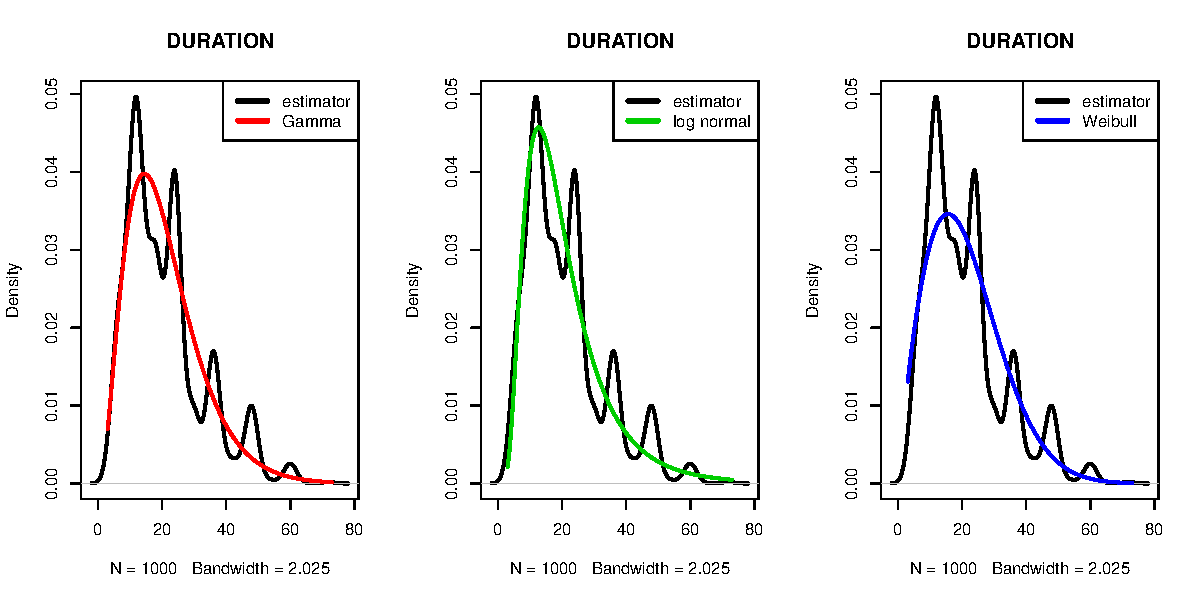
\includegraphics[width=.95\linewidth]{figure/unnamed-chunk-3-1} 

\end{knitrout}
\caption{Kernel density estimate of $DURATION$ variable density (black line) and curves representing density of the distribution fitted.}
\end{figure}

\begin{figure}[h!]
\centering
\begin{knitrout}
\definecolor{shadecolor}{rgb}{0.969, 0.969, 0.969}\color{fgcolor}\begin{kframe}


{\ttfamily\noindent\bfseries\color{errorcolor}{\#\# Error in stats::optim(x = c(1169, 5951, 2096, 7882, 4870, 9055, 2835, : non-finite finite-difference value [1]}}\end{kframe}
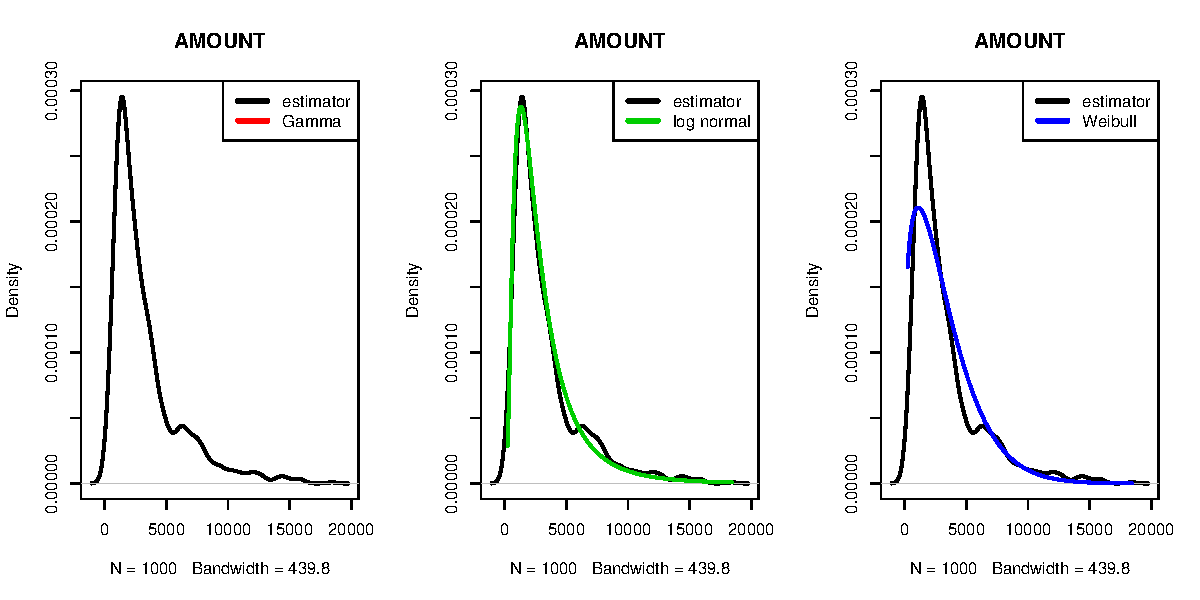
\includegraphics[width=.95\linewidth]{figure/unnamed-chunk-4-1} 

\end{knitrout}
\caption{Kernel density estimate of $AMOUNT$ variable density (black line) and curves representing density of the distribution fitted.}
\end{figure}


\begin{figure}[h!]
\centering
\begin{knitrout}
\definecolor{shadecolor}{rgb}{0.969, 0.969, 0.969}\color{fgcolor}
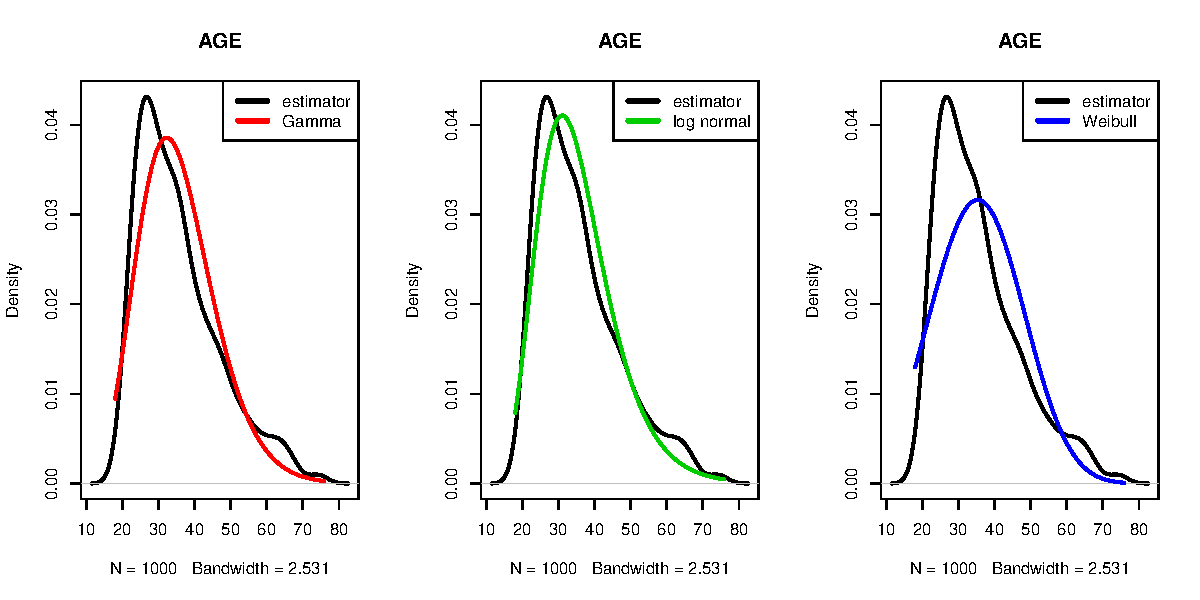
\includegraphics[width=.95\linewidth]{figure/unnamed-chunk-5-1} 

\end{knitrout}
\caption{Kernel density estimate of $AGE$ variable density (black line) and curves representing density of the distribution fitted.}
\end{figure}


\clearpage
\subsection{Creating derived variables}
\paragraph{}

We were considering possibilities of creating derived variables. We came up with propositions of the following formulas:
$$AMOUNT\_TO\_DURATION = AMOUNT / DURATION,$$
$$DURATION\_TO\_AGE = DURATION / AGE,$$
$$AMOUNT\_TO\_AGE = AMOUNT / AGE.$$

On the \textit{Figure 4.} we can see boxplots of $DURATION$, $AGE$ and $AMOUNT$ across two levels of response variable $RES$. On the \textit{Figure 5.} we can see boxplots of derived variables. This comparision can give us intuition how well our new variables separate good and bad bank clients.

\begin{figure}[h!]
\centering
\begin{knitrout}
\definecolor{shadecolor}{rgb}{0.969, 0.969, 0.969}\color{fgcolor}
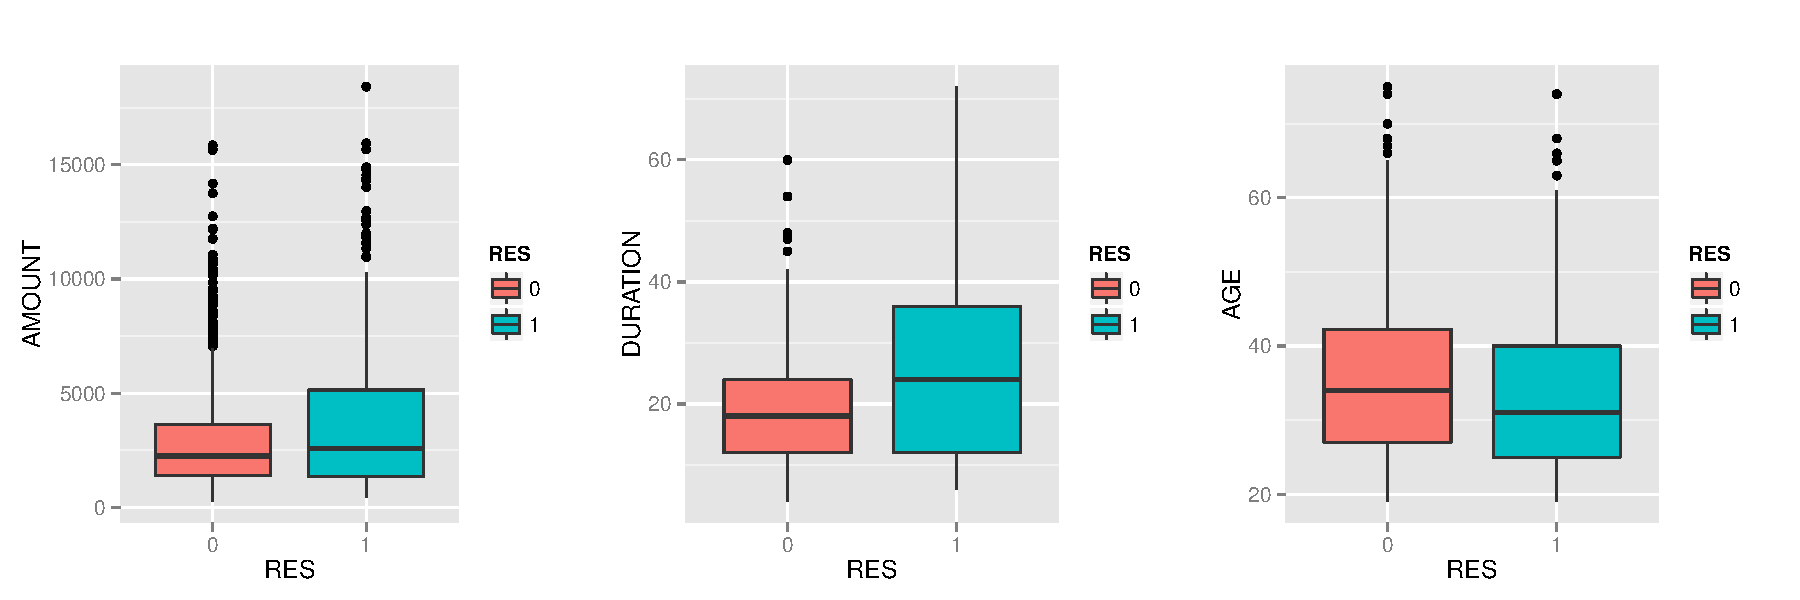
\includegraphics[width=.99\linewidth]{figure/unnamed-chunk-6-1} 

\end{knitrout}
\caption{Boxplots of $AMOUNT$, $DURATION$ and $AGE$ variables across two levels of response variable $RES$.}
\end{figure}

\begin{figure}[h!]
\centering
\begin{knitrout}
\definecolor{shadecolor}{rgb}{0.969, 0.969, 0.969}\color{fgcolor}
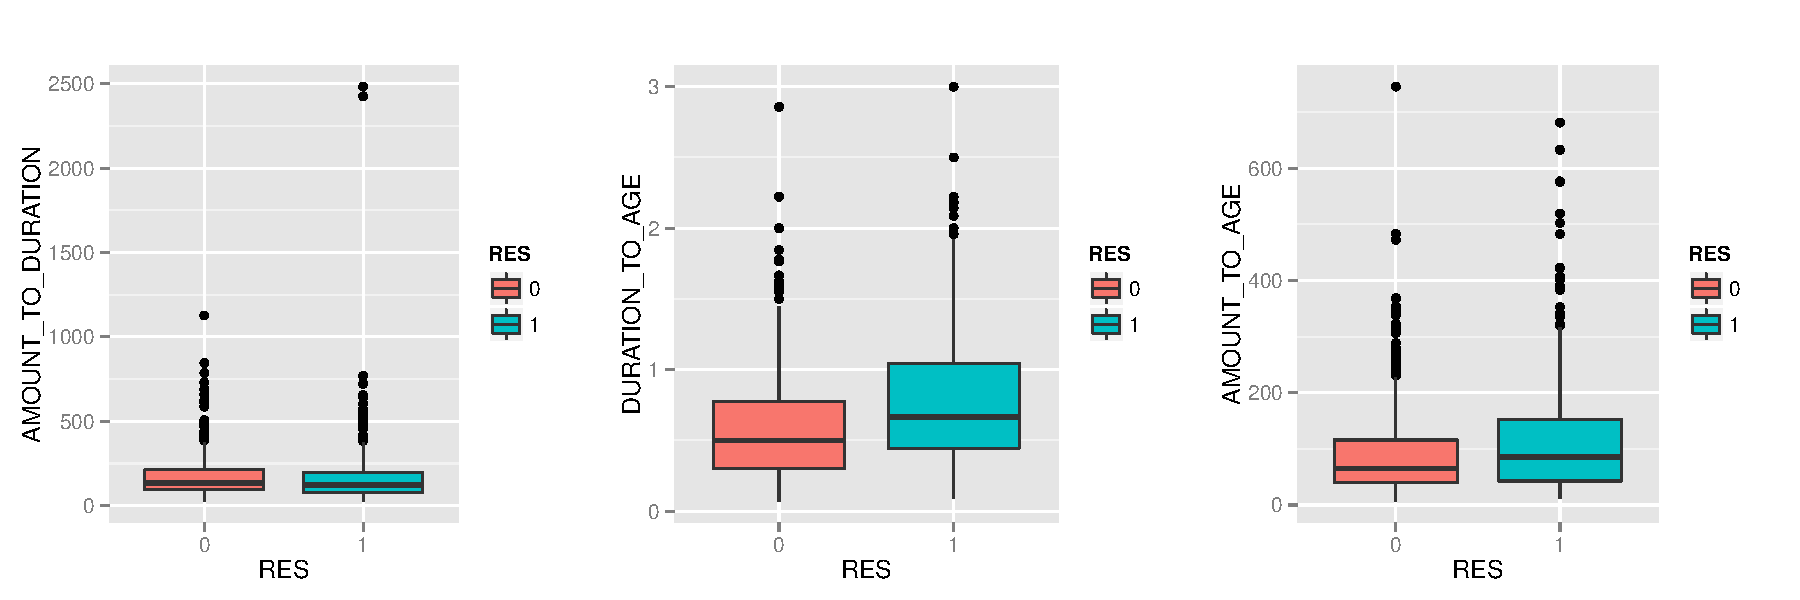
\includegraphics[width=.99\linewidth]{figure/unnamed-chunk-7-1} 

\end{knitrout}
\caption{Boxplots of derived variables: $AMOUNT\_TO\_DURATION$, $DURATION\_TO\_AGE$ and $AMOUNT\_TO\_AGE$ across two levels of response variable $RES$.}
\end{figure}

\paragraph{}
The boxplots on the \textit{Figure 5.} agree with our intuition: we expect higher $DURATION\_TO\_AGE$ and $AMOUNT\_TO\_AGE$ values for those clients who defaulted ($RES=1$). On the other hand, we would expect the same for the $AMOUNT\_TO\_DURATION$ variable whereas the plot shows something slightly opposite. However, the value differences on the $AMOUNT\_TO\_DURATION$ boxplot are so fine that we suppose this variable is going to turn out to be of low information value and will not be consider as important one. 

\subsection{Binning continuous variables}
\paragraph{}
In our analysis we compared three approaches of dividing continuous variables into categories: 
\begin{enumerate}
\item equal frequency discretization (resulted bins are of equal number of observations),
\item supervised discretization which utilizes Recursive Partitioning to categorize the numeric characteristic and compute cutpoins based on Conditional Inference Trees algorithm ($smbinning$ package),
\item categorize variable with simple tree model (from $rpart$ package, with the use of default tree building parameters).
\end{enumerate}

The IV comparision is presented on the \textit{Figure 6.} below. Note that equal frequency discretization results are presented for:
\begin{itemize}
\item the same number of bins as in variable resulted from $smbinning$ method; signature: $equal\_nbins$,
\item the same number of bins as in variable resulted from $rpart$ method; signature: $equal\_nrparts$.
\end{itemize}



\begin{figure}[h!]
\centering
\begin{knitrout}
\definecolor{shadecolor}{rgb}{0.969, 0.969, 0.969}\color{fgcolor}
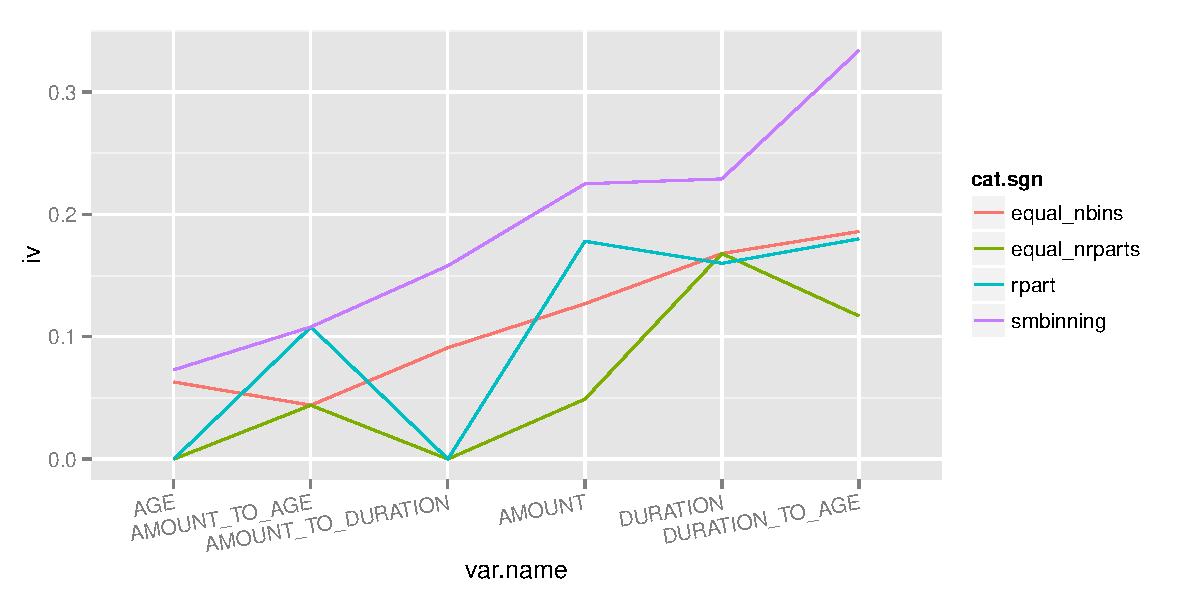
\includegraphics[width=.95\linewidth]{figure/unnamed-chunk-9-1} 

\end{knitrout}
\caption{Comparision of Information Values of variables resulted from binning performed by means of 3 differend approaches. }
\end{figure}

We can see a few interesting things from the plot above: 
\begin{itemize}
\item The $smbinning$ function from the $smbinning$ seems to beat other methods in terms of IV of resulted binned variable. 
\item Derived variable $DURATION\_TO\_AGE$ has a strong relationship to the Goods/Bads odds ratio (over 0.33 IV value), whereas two other derived variables ($AMOUNT\_TO\_AGE$, $AMOUNT\_TO\_DURATION$) seem to have not. 
\end{itemize}


\subsection{Correcting bins (levels) of categorical variables}
\paragraph{}
The last element of data pre-processing we performet os correcting bins (levels) of categorical variables. In the domain of particular variable's levels, we searched for levels which: 
\begin{itemize}
\item reasonalby similar in terms of their meaning (e.g. for $PURPOSE$ variable we have logically similar levels: \textit{car (new)} and \textit{car (old)},
\item do not vary in terms of $GOOD$ / $BAD$ observations fraction.
\end{itemize}
\paragraph{}
To assess whether or not levels vary in terms of $GOOD$ / $BAD$ observations fraction we wrote a function which compute Information Value for non-changed variable and the same variable with a par of levels joined, for all possible pair of levels. Below we present the head table output of this function and WoE plot for each of the levels for a particular variable.
\paragraph{}
We include results for the two variables in case of which we decided to perform bin correcting. 

\begin{enumerate}
\item $PURPOSE$



Below we can see what is the $PURPOSE$ variable IV ($3^{rd}$ column) after joining a pair of levels ($1^{st}$ and $2^{nd}$ column). 

\begin{knitrout}
\definecolor{shadecolor}{rgb}{0.969, 0.969, 0.969}\color{fgcolor}
\begin{tabular}{l|l|l|r}
\hline
  & lvl1 & lvl2 & iv\\
\hline
46 & NONE & NONE & 0.1692\\
\hline
21 & furniture/equipment & domestic appliances & 0.1692\\
\hline
37 & business & repairs & 0.1691\\
\hline
36 & business & domestic appliances & 0.1691\\
\hline
16 & education & others & 0.1691\\
\hline
28 & car (new) & repairs & 0.1691\\
\hline
\end{tabular}


\end{knitrout}

We can also investigate the WoE values plot: 

\begin{knitrout}
\definecolor{shadecolor}{rgb}{0.969, 0.969, 0.969}\color{fgcolor}
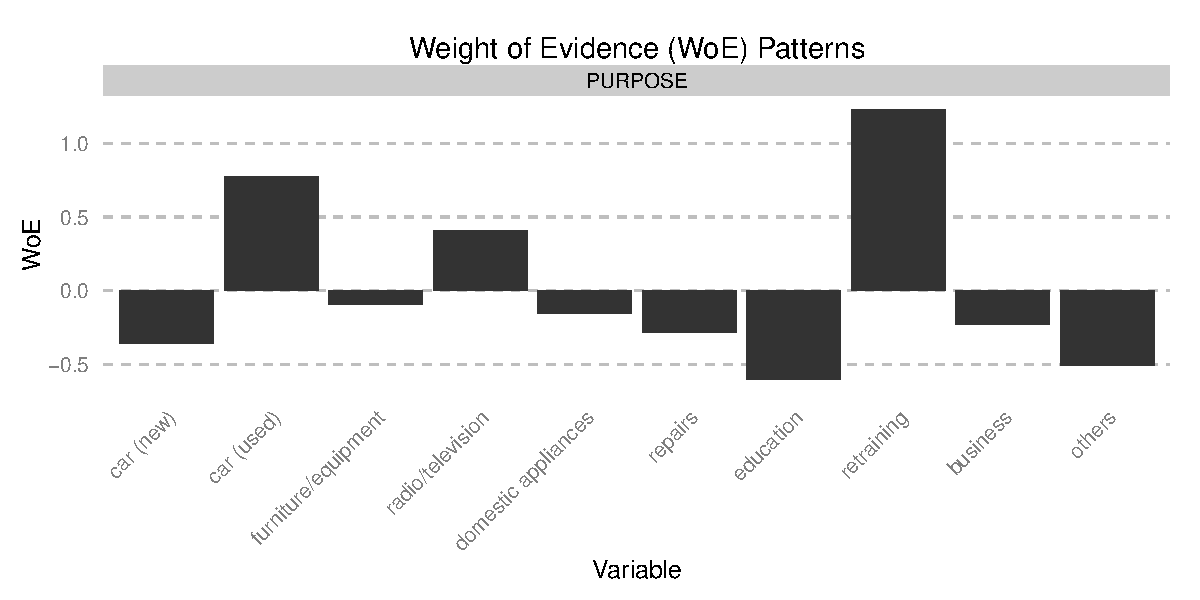
\includegraphics[width=.65\linewidth]{figure/unnamed-chunk-12-1} 

\end{knitrout}

Judging from the above study we concluded that it is reasonable to join $furniture/equipment$ and $domestic appliances$ levels and we performed it. 

\item $HOUSING$



Below we can see what is the $HOUSING$ variable IV ($3^{rd}$ column) after joining a pair of levels ($1^{st}$ and $2^{nd}$ column). 

\begin{knitrout}
\definecolor{shadecolor}{rgb}{0.969, 0.969, 0.969}\color{fgcolor}
\begin{tabular}{l|l|l|r}
\hline
  & lvl1 & lvl2 & iv\\
\hline
4 & NONE & NONE & 0.0833\\
\hline
3 & for free & rent & 0.0830\\
\hline
1 & own & for free & 0.0389\\
\hline
2 & own & rent & 0.0296\\
\hline
\end{tabular}


\end{knitrout}

We can also investigate the WoE values plot: 

\begin{knitrout}
\definecolor{shadecolor}{rgb}{0.969, 0.969, 0.969}\color{fgcolor}
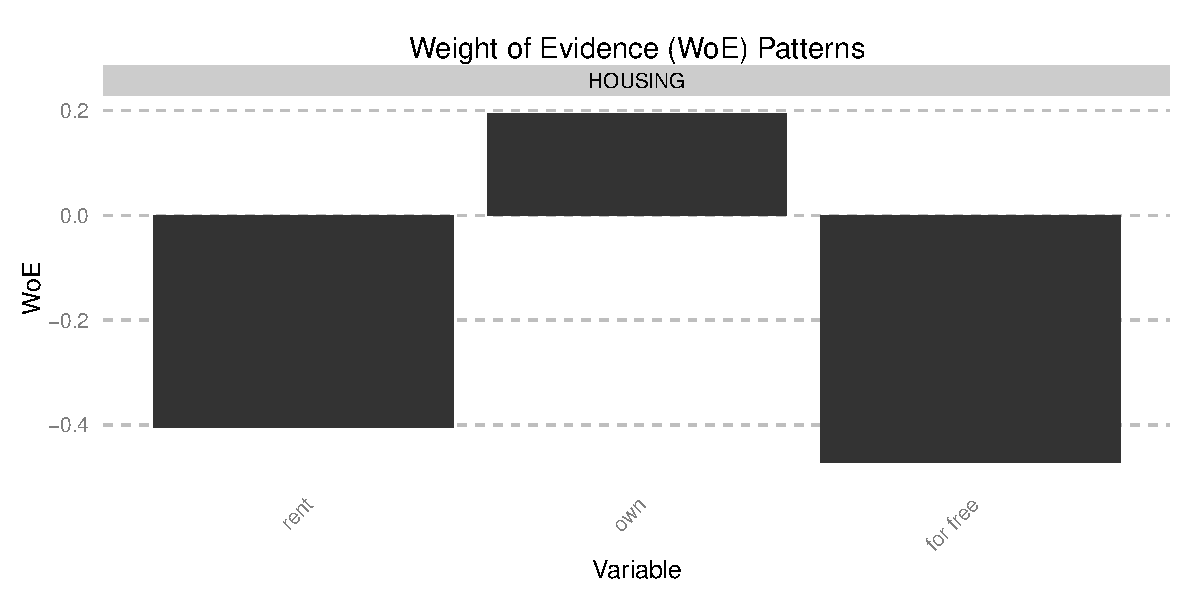
\includegraphics[width=.65\linewidth]{figure/unnamed-chunk-15-1} 

\end{knitrout}

Judging from the above study we concluded that it is reasonable to join $for free$ and $rent$ levels and we performed it. 
\end{enumerate}


\subsection{Removing variables of $0.0$ Information Value}
\paragraph{}
After the transformations described above, we chcecked what are IV for each of the resulting variable. The values are presented below.




\begin{knitrout}
\definecolor{shadecolor}{rgb}{0.969, 0.969, 0.969}\color{fgcolor}
\begin{tabular}{l|r|r|r|l}
\hline
Variable & InformationValue & Bins & ZeroBins & Strength\\
\hline
CHK\_ACCT & 0.6660 & 4 & 0 & Very strong\\
\hline
DURATION\_TO\_AGE & 0.3338 & 3 & 0 & Strong\\
\hline
HISTORY & 0.2932 & 5 & 0 & Strong\\
\hline
DURATION & 0.2293 & 3 & 0 & Strong\\
\hline
AMOUNT & 0.2251 & 4 & 0 & Strong\\
\hline
SAVINGS\_ACCT & 0.1960 & 5 & 0 & Average\\
\hline
PURPOSE & 0.1692 & 9 & 0 & Average\\
\hline
AMOUNT\_TO\_DURATION & 0.1575 & 5 & 0 & Average\\
\hline
PROPERTY & 0.1126 & 4 & 0 & Average\\
\hline
AMOUNT\_TO\_AGE & 0.1082 & 2 & 0 & Average\\
\hline
EMLOYMENT & 0.0864 & 5 & 0 & Weak\\
\hline
HOUSING & 0.0830 & 2 & 0 & Weak\\
\hline
AGE & 0.0732 & 2 & 0 & Weak\\
\hline
OTHER\_INSTALLMENT\_PLANS & 0.0576 & 3 & 0 & Weak\\
\hline
STATUS\_AND\_SEX & 0.0447 & 4 & 0 & Weak\\
\hline
IS\_FOREIGN\_WORKER & 0.0439 & 2 & 0 & Weak\\
\hline
OTHER\_DEBTORS & 0.0320 & 3 & 0 & Weak\\
\hline
RATE\_TO\_DISP\_INCOME & 0.0239 & 2 & 0 & Weak\\
\hline
NUM\_OF\_THIS\_BANK\_CREDITS & 0.0101 & 2 & 0 & Wery weak\\
\hline
JOB & 0.0081 & 3 & 0 & Wery weak\\
\hline
TELEPHONE & 0.0064 & 2 & 0 & Wery weak\\
\hline
NUM\_OF\_MAINTAINED\_PEOPLE & 0.0000 & 1 & 0 & Wery weak\\
\hline
RESIDENCE & 0.0000 & 1 & 0 & Wery weak\\
\hline
\end{tabular}


\end{knitrout}

We can see that two variables: $NUM\_OF\_MAINTAINED\_PEOPLE$ and $RESIDENCE$ have $0.0$ information value. We decided to remove them from the data set as we assume they are kind of useless data.


\subsection{Recoding variables to WoE}
\paragraph{}
After the operations descripted above, we made a copy of our data and converted all of the categorical variables in this copy into their WoE representatives. Since then 
we have been working on two data sets: 
\begin{enumerate}
\item \textit{german\_data\_cat.txt} - categorized data set,
\item \textit{german\_data\_woe.txt} - categorized and recoded to WoE data set (besides the response variable, this data set contains numeric variables only). 
\end{enumerate}


\subsection{Data preprocessing summary}
\paragraph{}
To conclude, the data preprocessing we performed above results in: 
  \begin{itemize}
\item creating derived variables and including them into the data set: $AMOUNT\_TO\_DURATION$, $DURATION\_TO\_AGE$ and $AMOUNT\_TO\_AGE$,
\item binning continuous variables with the use of \textit{smbinning} method and keeping them in those binned form in the data set; related to: $AGE$, $AMOUNT$, $DURATION$, $AMOUNT\_TO\_DURATION$, $DURATION\_TO\_AGE$ and $AMOUNT\_TO\_AGE$,
\item correcting bins (levels) of categorical variables and keeping them in those transformed form in the data set: $PURPOSE$ and $HOUSING$,
\item removing variables of $0.0$ information value:  $NUM\_OF\_MAINTAINED\_PEOPLE$ and $RESIDENCE$,
\item creating separated data set which contains all the categorical variables in the recoded to WoE form. 
\end{itemize}





% ==============================================================================
% ==============================================================================
% ==============================================================================
\clearpage
\section{Feature Selection}


\subsection{Filter comparison}
\begin{figure}[h!]
  \centering
  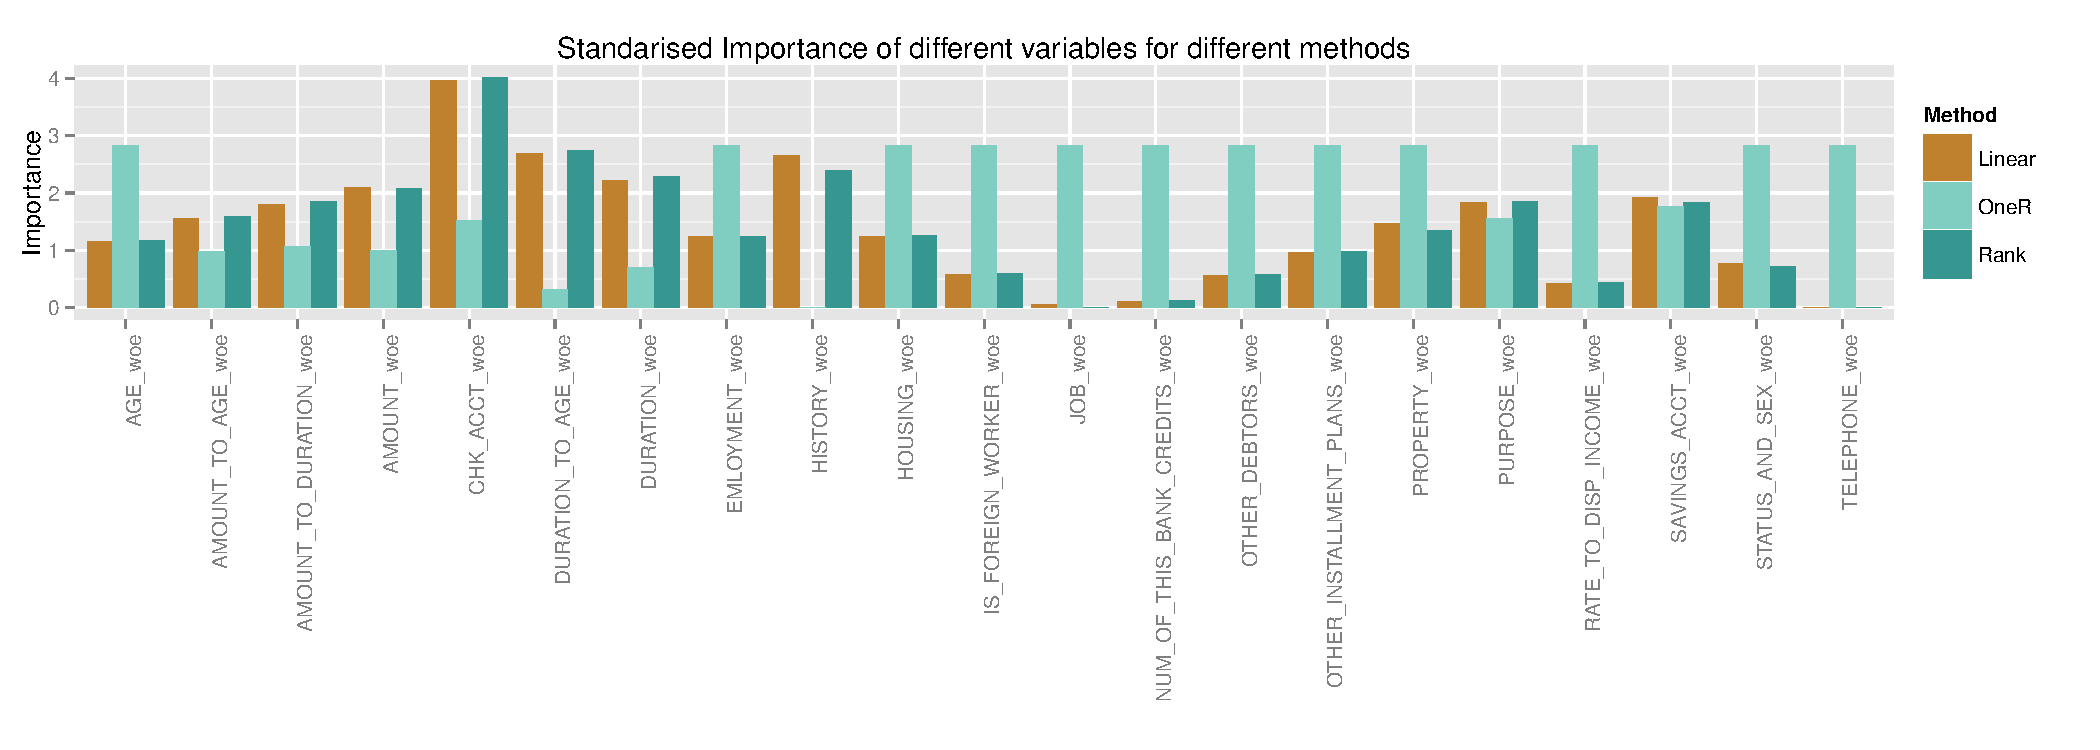
\includegraphics[width=0.9\textwidth]{Plots/Rplot03}
  \caption[Close up of \textit{Hemidactylus} sp.]
   {Histogram of the importance of different variables for woe transformation data}
\end{figure}

There had been involved many measures of the variable importance. Most of them
are giving similar results. The most important Variable seems to be CHK\_ACCT and the least important variables such as: IS\_FOREIGN\_WORKER (which is for 0.95 cases constant), TELEPHONE or JOB. Linear and Rank corelation methods gave also some idea about correlation WOE transformation of the data with the response variable.

\begin{figure}[h!]
  \centering
  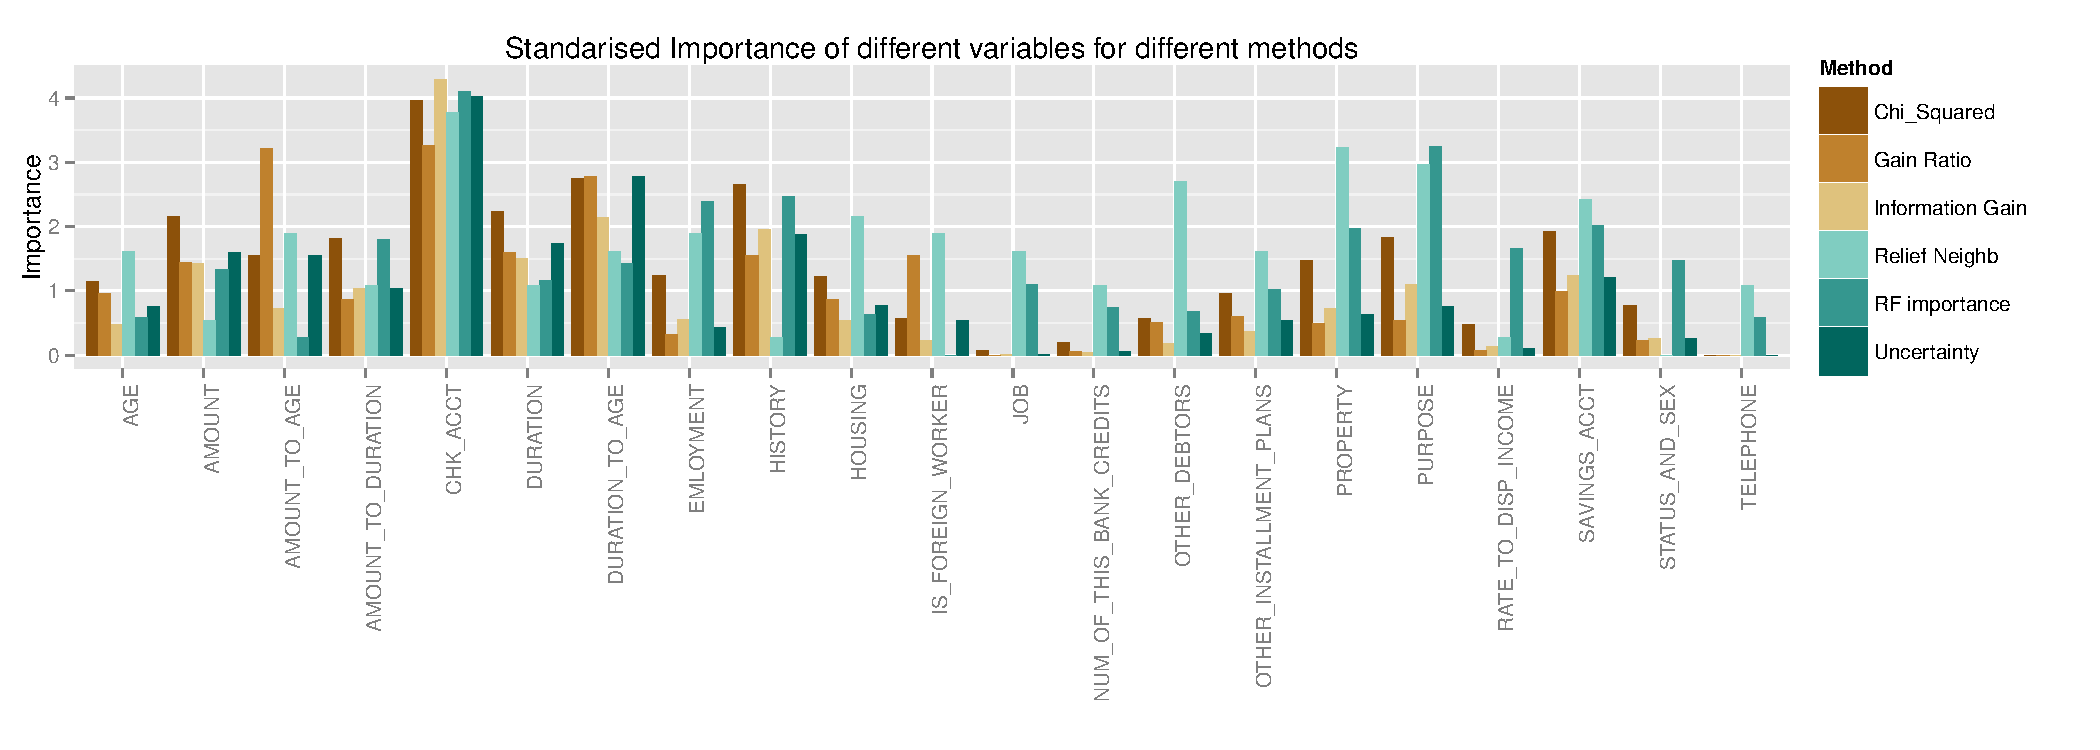
\includegraphics[width=0.9\textwidth]{Plots/Rplot04}
  \caption[Close up of \textit{Hemidactylus} sp.]
   {Histogram of the importance of different variables for categorical data}
\end{figure}

However most of the results for the diffenert  methods are similar, some might be interesting. For example high contribution of the variables PURPOSE and PROPERTY difrenciate RF importance and eighbarhood methods from the others. 


\clearpage

\subsection{Models without features selection}




\begin{table}[ht]
\centering
\begin{tabular}{rlrrrrrr}
\hline
& Label & ACC & TPR & SPC & PPV & F1 & FDR \\ 
\hline
1 & Boosting & 0.79 & 0.81 & 0.69 & 0.90 & 0.85 & 0.10 \\ 
2 & Random Forest & 0.76 & 0.78 & 0.67 & 0.91 & 0.84 & 0.09 \\ 
3 & AIC Logistic regression & 0.78 & 0.82 & 0.65 & 0.88 & 0.85 & 0.12 \\ 
4 & Logistic regression & 0.78 & 0.82 & 0.67 & 0.88 & 0.85 & 0.12 \\ 
5 & K-NN & 0.80 & 0.84 & 0.67 & 0.89 & 0.87 & 0.11 \\ 
6 & Linear Dyscryminant Analysis & 0.78 & 0.83 & 0.63 & 0.88 & 0.85 & 0.12 \\ 
7 & Quadric Dyscriminant Analysis & 0.78 & 0.87 & 0.59 & 0.82 & 0.84 & 0.18 \\ 
\hline
\end{tabular}
\caption{Basic statistics for models with all features} 
\end{table}

First step in the modeling part for this case had been fitting simple models for all features. It had been expected that soe of the methods would perform well under this constraints, as long as they have its own feature selection methodology. One of such methods is Random Forest. Suprisingly it had just 0.76 Accuracy. Method that were supposed to perform not to good (KNN) had extremally good Accuracy of 0.8. 



\subsection{CSF method}

\begin{table}[ht]
\centering
\begin{tabular}{rlrrrrrr}
\hline
& Label & ACC & TPR & SPC & PPV & F1 & FDR \\ 
\hline
1 & AIC Logistic Regression & 0.76 & 0.82 & 0.60 & 0.83 & 0.83 & 0.17 \\ 
2 & Logistic Regression & 0.75 & 0.76 & 0.66 & 0.93 & 0.84 & 0.07 \\ 
3 & K-NN & 0.76 & 0.79 & 0.59 & 0.90 & 0.84 & 0.10 \\ 
4 & Linear Dyscriminant Analysis & 0.78 & 0.83 & 0.61 & 0.87 & 0.85 & 0.13 \\ 
5 & Quadric Dyscriminant Analysis & 0.80 & 0.84 & 0.65 & 0.88 & 0.86 & 0.12 \\ 
\hline
\end{tabular}
\caption{Basic statistics for models with features from CFS method} 
\end{table}

First regular method of subset selection had been CFS. Is gave conservative results of just few features for models:
\begin{itemize}
\item DURATION\_TO\_AGE, CHK\_ACCT HISTORY and SAVINGS\_ACCT for WOE transformation of the data
\item DURATION\_TO\_AGE, CHK\_ACCT and HISTORY categoregorical data
\end{itemize}

At this place interesting observation is that only 3 or 4 variables could give almost the same Accuracy as 21. According to Razor rule eventhough there is a small diffenence in the performance f the models, preffered would be those with much less predictors. QDA results with the accuracy 0.8 are even similar to those resulted from KNN using all variables.

\clearpage

\subsection{Consistency method}

\begin{table}[ht]
\centering
\begin{tabular}{rlrrrrrr}
\hline
& Label & ACC & TPR & SPC & PPV & F1 & FDR \\ 
\hline
1 & AIC Logistic Regression & 0.81 & 0.83 & 0.72 & 0.90 & 0.87 & 0.10 \\ 
2 & Logistic Regression & 0.80 & 0.83 & 0.71 & 0.90 & 0.86 & 0.10 \\ 
3 & K-NN & 0.79 & 0.83 & 0.63 & 0.88 & 0.86 & 0.12 \\ 
4 & Linear Dyscriminant Analysis & 0.81 & 0.84 & 0.70 & 0.91 & 0.87 & 0.09 \\ 
5 & Quadric Dyscriminant Analysis & 0.79 & 0.83 & 0.64 & 0.88 & 0.86 & 0.12 \\ 
\hline
\end{tabular}
\caption{Basic statistics for models with features from consistency method} 
\end{table}

Using consistency method there had been another set obtained. This time more quantitative. 

\begin{itemize}

\item DURATION, AMOUNT, AMOUNT\_TO\_DURATION, DURATION\_TO\_AGE, 
    AMOUNT\_TO\_AGE, PURPOSE, CHK\_ACCT, HISTORY, 
    SAVINGS\_ACCT for WOE transformation of the data
    
\item RATE\_TO\_DISP\_INCOME, NUM\_OF\_THIS\_BANK\_CREDITS, AGE, 
    DURATION\_TO\_AGE, PURPOSE, CHK\_ACCT, HISTORY, SAVINGS\_ACCT, 
    EMLOYMENT,  JOB , OTHER\_DEBTORS, PROPERTY and STATUS\_AND\_SEX for categoregorical data
\end{itemize}

This time results are better than ever before. It shows the importance of the feature selection during the model fitting process. 

\subsection{Best subset method}



\begin{figure}[h!]
  \centering
  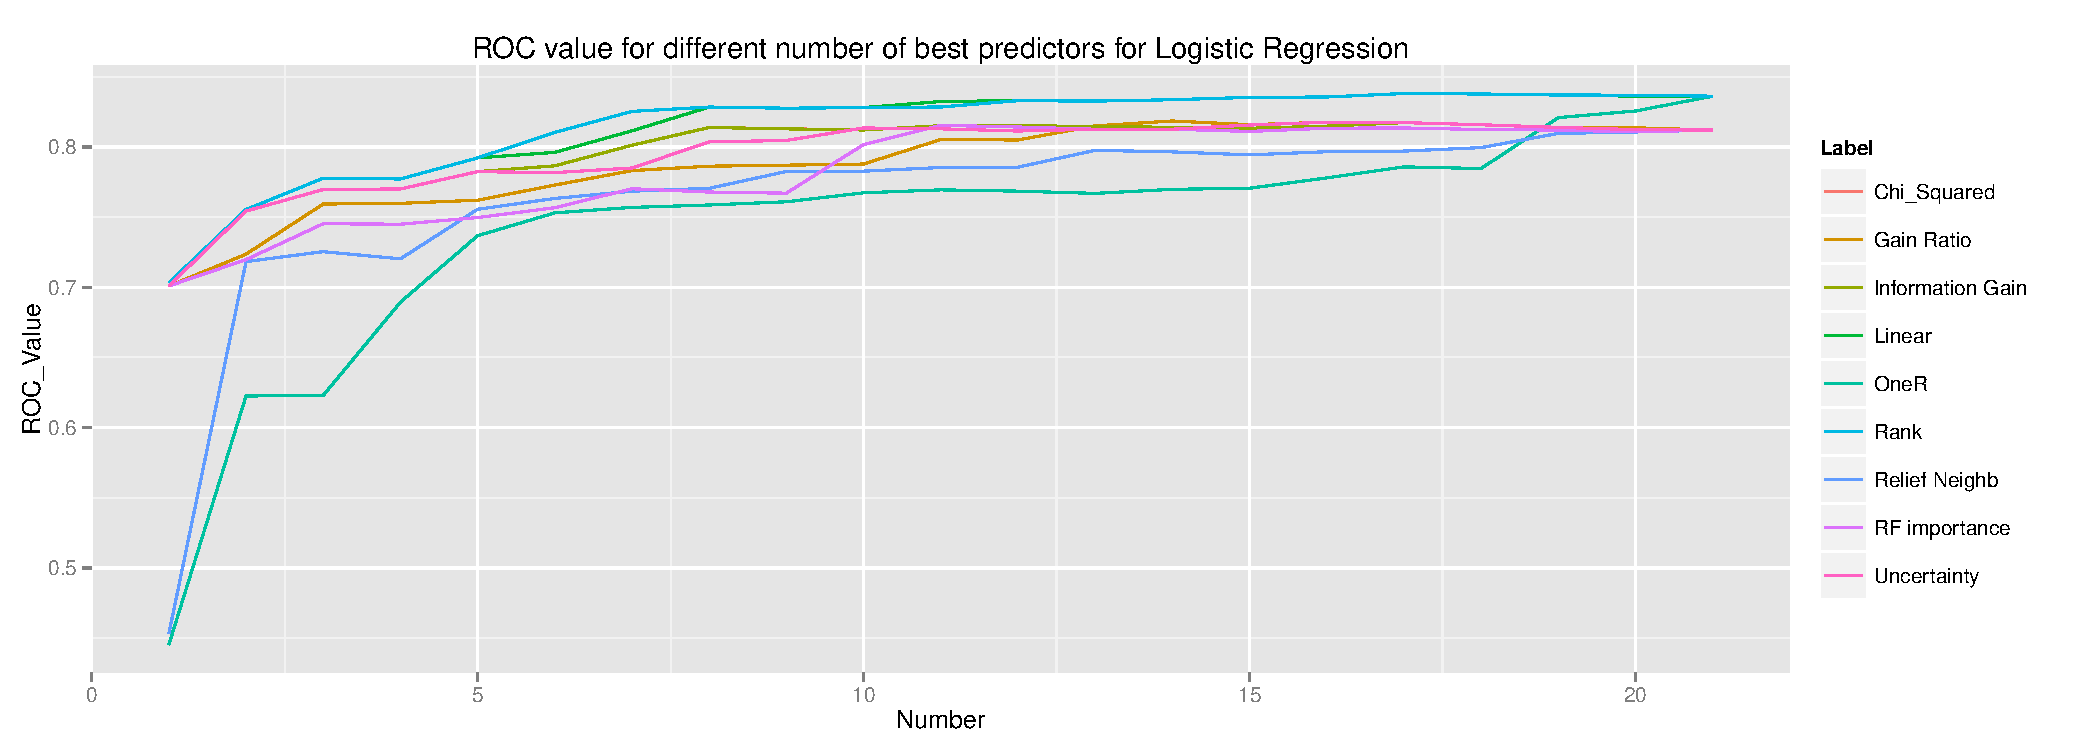
\includegraphics[width=0.8\textwidth]{Plots/Rplot}
  \caption[Close up of \textit{Hemidactylus} sp.]
   {Comparison of the first n best variables for different methods using GLM model}
\end{figure}

We developed another method to choice the best and moderately big subset for modeling. Using all filters from the first subsection we went to show how good results would be acheived using just first n best predictors for given measure. 
Results are interesting. For some algorythms the adequate maximum is achieved for relatively small number of predictors. 
We choose subset having only 8 predictors based on Information gain. In following paragraphs we would see how does it work for different algorithms.

\clearpage

\begin{table}[ht]
\centering
\begin{tabular}{rlrrrrrr}
\hline
& Label & ACC & TPR & SPC & PPV & F1 & FDR \\ 
\hline
1 & Logistic Regression & 0.81 & 0.84 & 0.72 & 0.90 & 0.87 & 0.10 \\ 
2 & K-NN & 0.79 & 0.82 & 0.66 & 0.90 & 0.86 & 0.10 \\ 
3 & Linear Dyscriminant Analysis & 0.80 & 0.84 & 0.66 & 0.89 & 0.86 & 0.11 \\ 
4 & Quadric Dyscriminant Analysis & 0.79 & 0.86 & 0.63 & 0.86 & 0.86 & 0.14 \\ 
\hline
\end{tabular}
\caption{Basic statistics for models with features from filtered best method} 
\end{table}

First important and interesting information is that using consistency rule and best subset for the AIC based Logistic Regression we got the same results. They would be discussed more in next paragraphs.




\section{Classification modelling results}
\subsection{Analysis of fitted models}


At first we would show some comparison analysis between some of the fitted models. In the next sections there would be discussed each model separately. 
Interesting observation is that Random Forest lost a lot comparing to the Boosting model (GBM). Rest of the algorithms at first looks as tough the results are similar. 

\begin{figure}[h!]
  \centering
  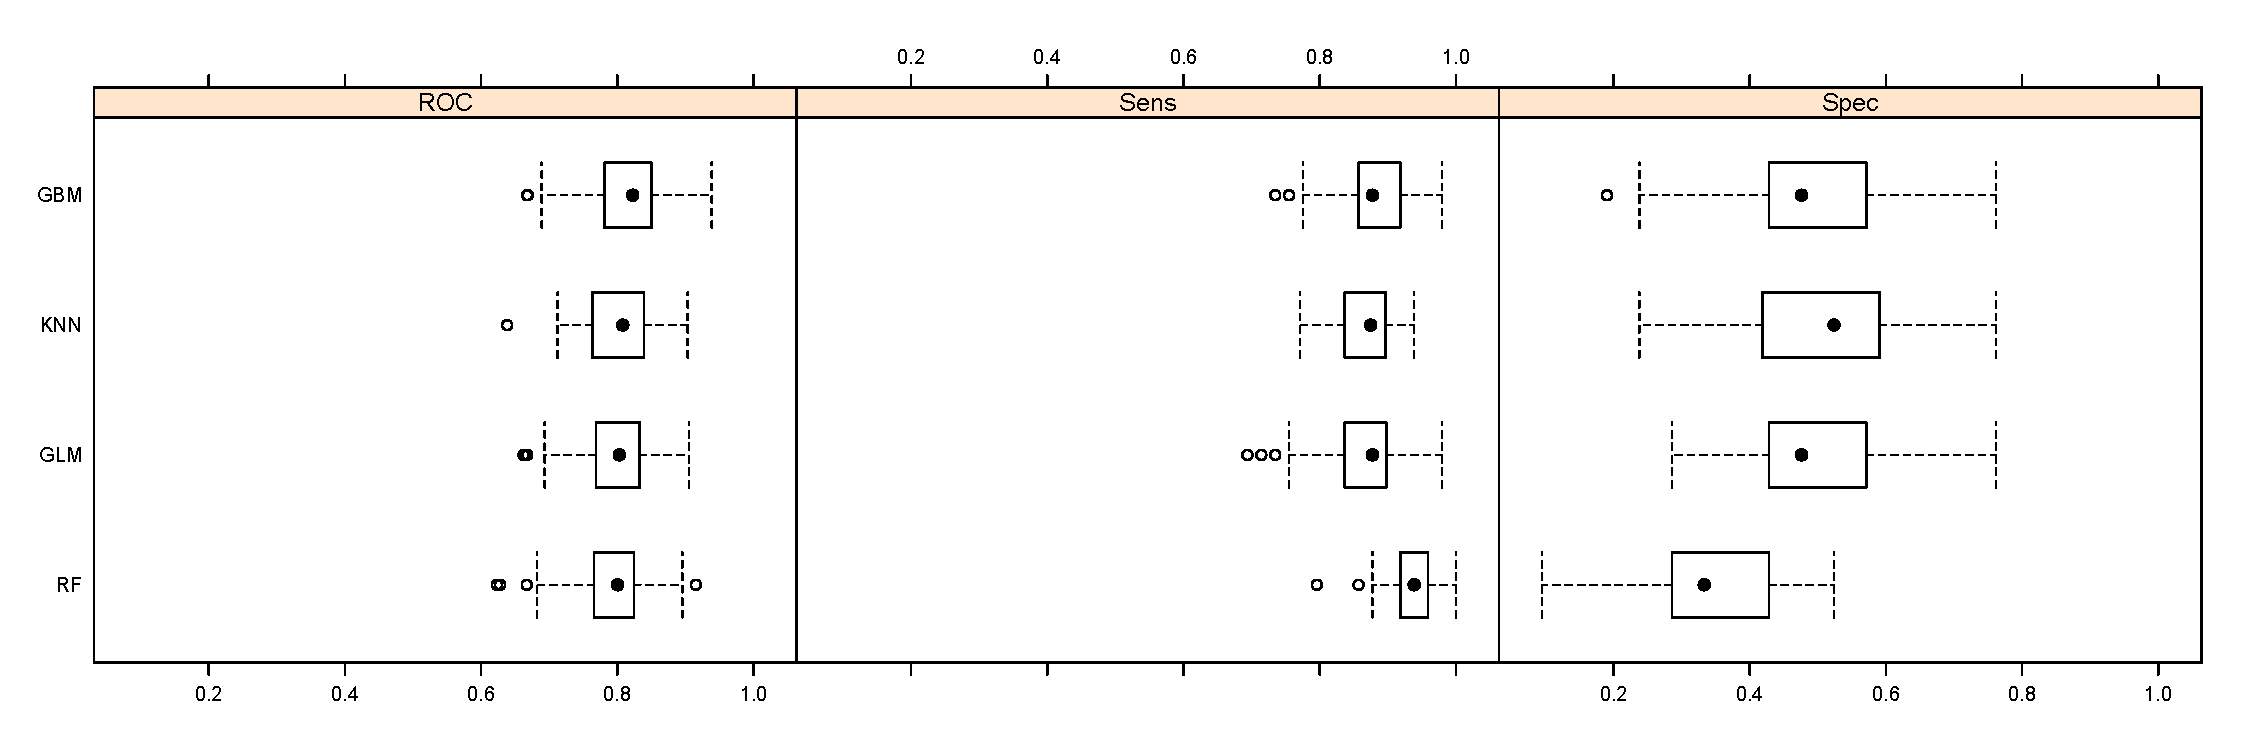
\includegraphics[width=0.9\textwidth]{Plots/STATS_MODEL_COMPARE}
  \caption[Close up of \textit{Hemidactylus} sp.]
   {Histogram of the importance of different variables for categorical data}
\end{figure}

Here are boxplots of the ROC values, Sensitiviti, and Specifity. It had been calculated using 10 times 10-fold classification for all models. It looks like most of the models have similar statistics besides Specifity and Sensitivity for Random Forest. Given good values for Sensitivity it looses some value on the second index.


\begin{figure}[h!]
  \centering
  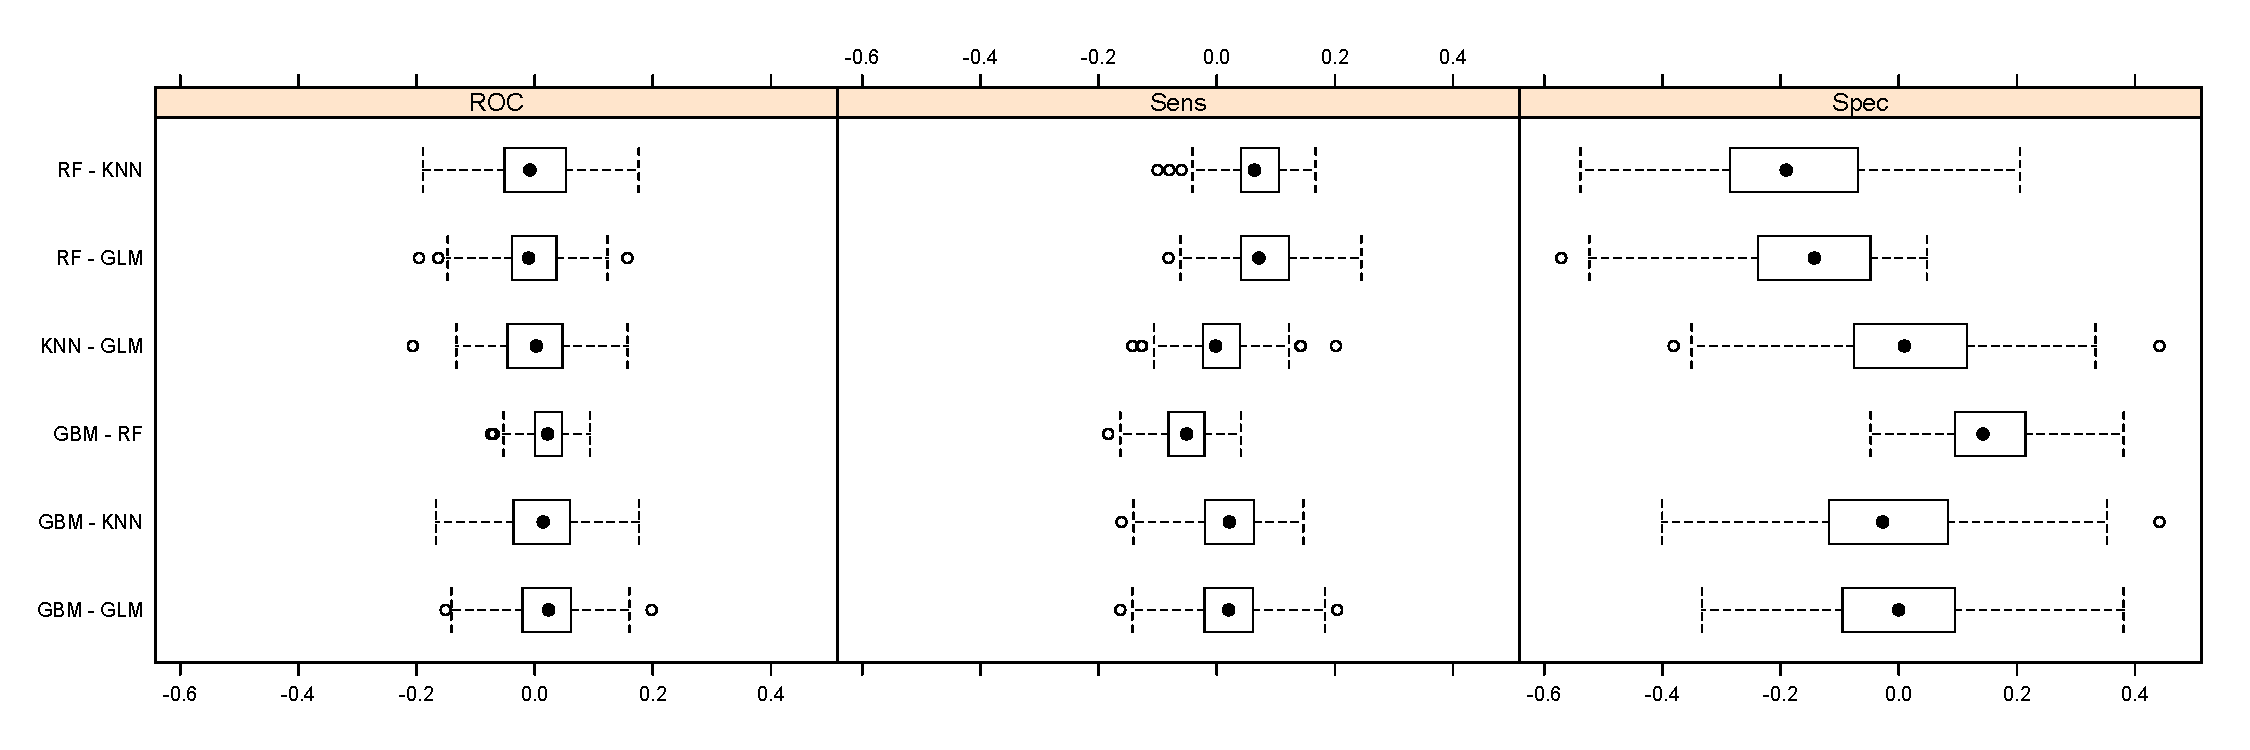
\includegraphics[width=0.9\textwidth]{Plots/STATS_DIF_MODEL_COMPARE}
  \caption[Close up of \textit{Hemidactylus} sp.]
   {Comparison of the first n best variables for different methods using GLM model}
\end{figure}



\begin{figure}[h!]
  \centering
  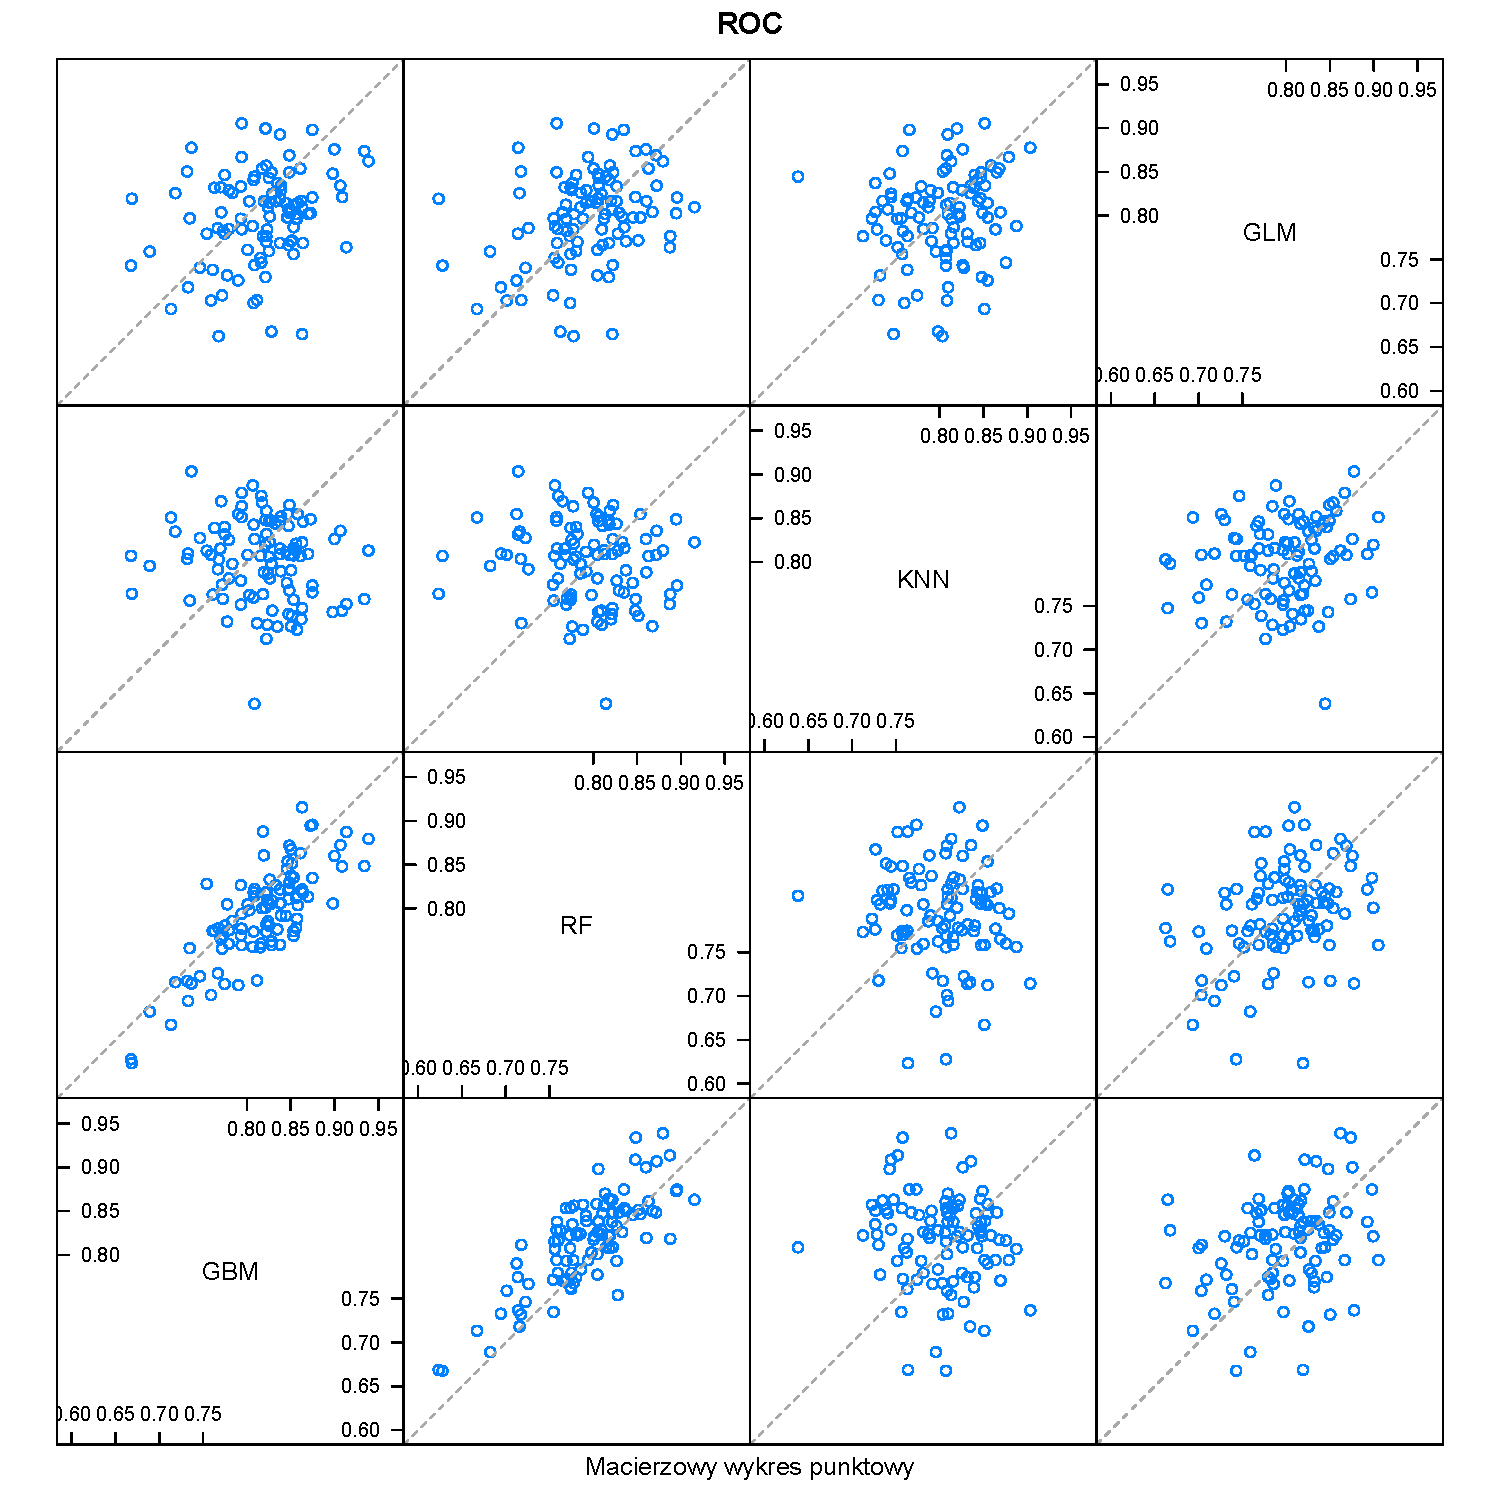
\includegraphics[width=0.8\textwidth]{Plots/SCATTER_MODEL_COMPARE}
  \caption[Close up of \textit{Hemidactylus} sp.]
   {Histogram of the importance of different variables for woe transformation data}
\end{figure}





Nonetheless Random Forest looks worse at first sight, the values of the ROC are very simmilar to the Boosting model. The biggest skeewnes is visible for Spec and Sens for those two models. There are differences in the classifications. That could suggest that usage of ensemble method could effect in improvement of the model performance. 


\clearpage

\subsection{Logistic Regression}

Logistic regression is the model that is used in industrie the most often. As it had been said before it thanks its popularity to easiness in interpretation of the results. Based oon this approach it is possible to produce scorecard which could be used to clasiffy approprietly cases. 

\begin{figure}[h!]
  \centering
  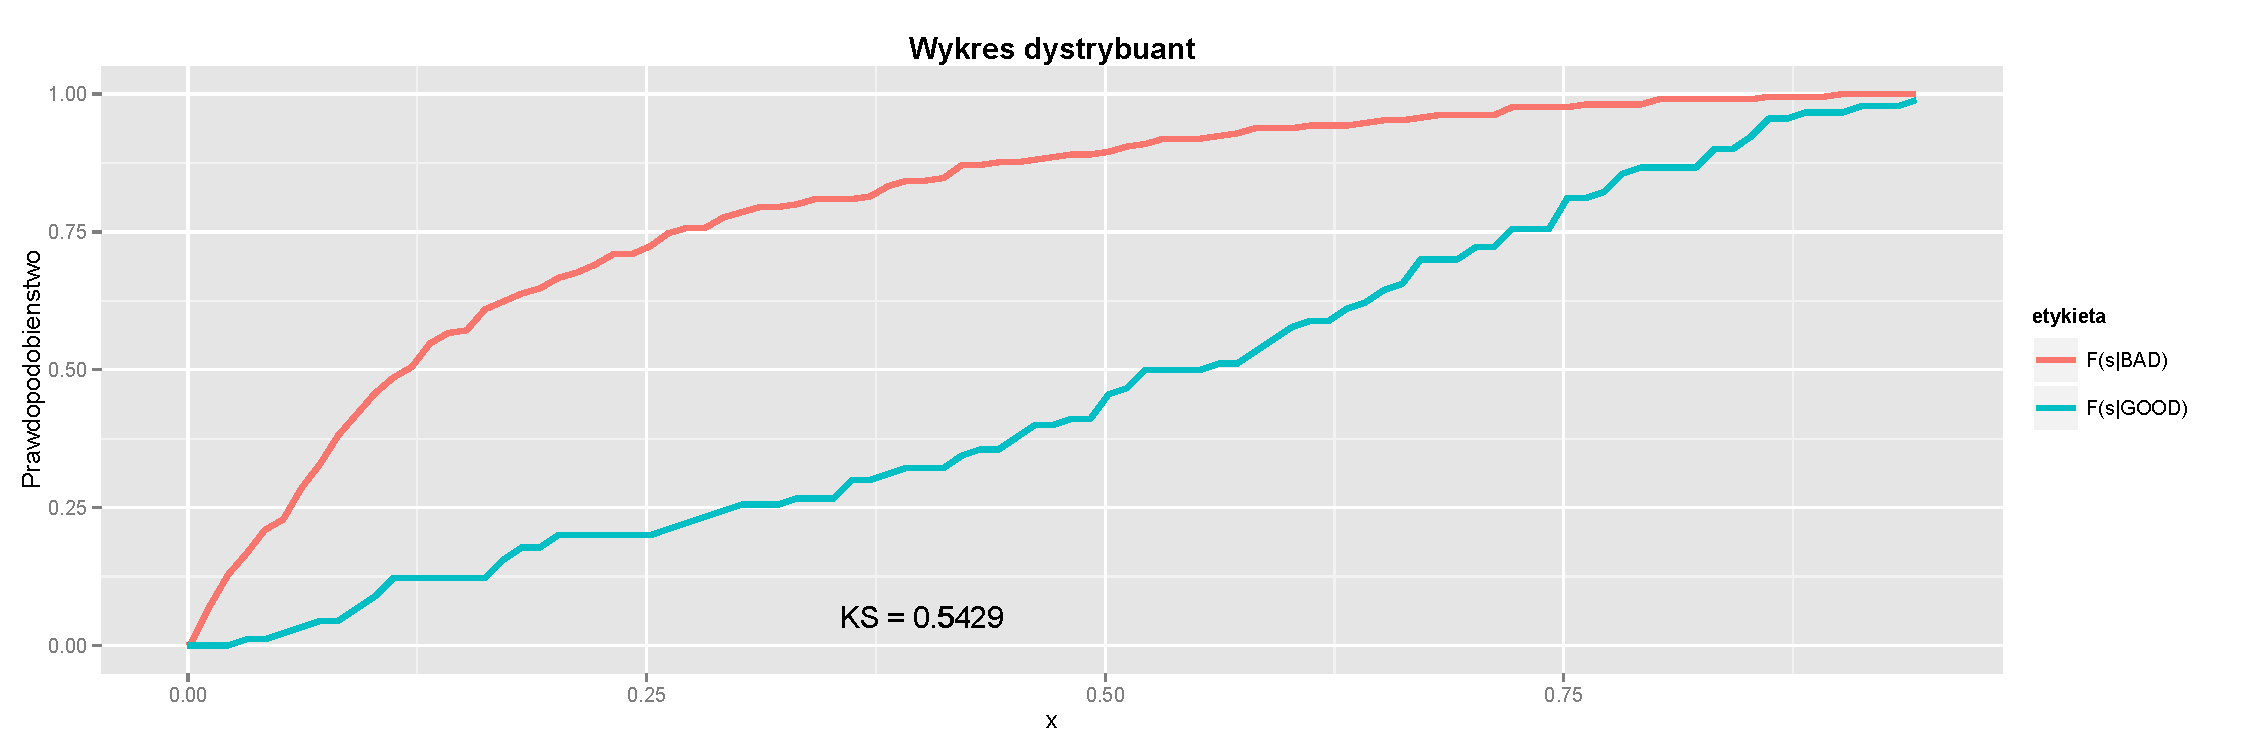
\includegraphics[width=0.9\textwidth]{Plots/GLM_KS}
  \caption[Close up of \textit{Hemidactylus} sp.]
   {Distribution plot for good and Bad class with KS statistic for GLM method}
\end{figure}

Plot abowe shows distributions for good and bad cases. The KS- statistics is high. That indicates good separation between classes for this particular model. 

\begin{figure}[h!]
        \centering
        \begin{subfigure}[b]{0.45\textwidth}
                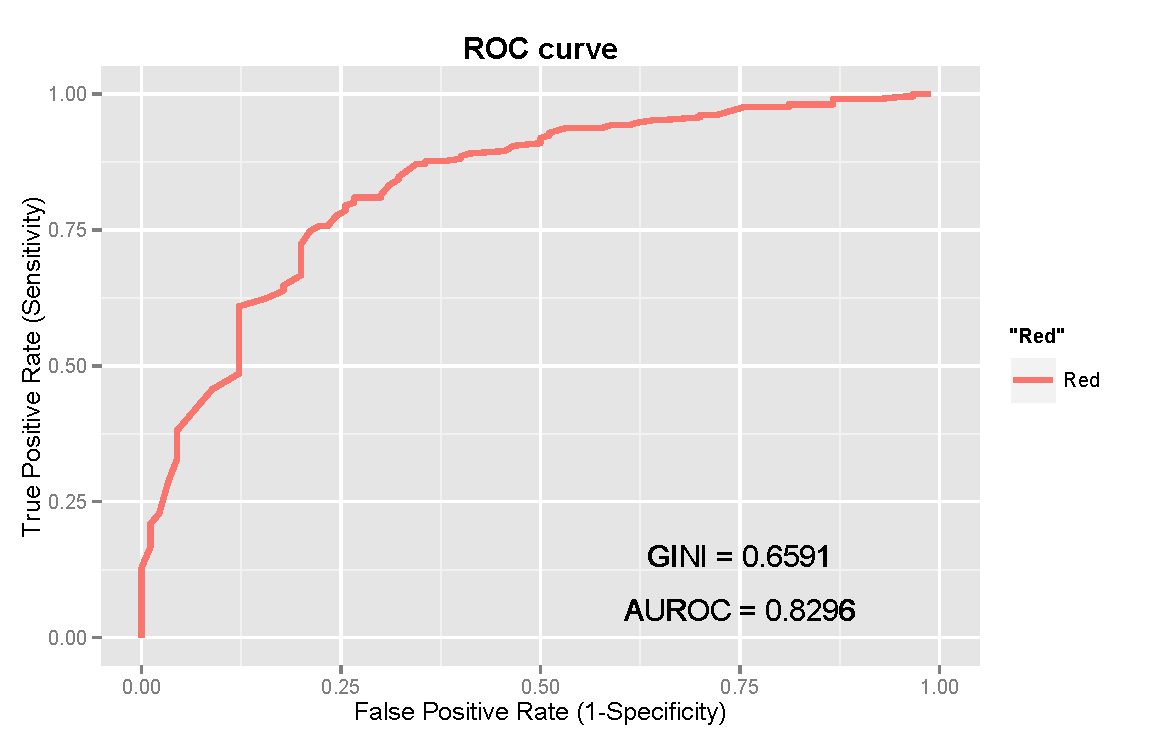
\includegraphics[width=\textwidth]{Plots/ROC_GLM}
                \caption{}
                \label{fig:ROC_ GLM}
        \end{subfigure}
        \begin{subfigure}[b]{0.45\textwidth}
                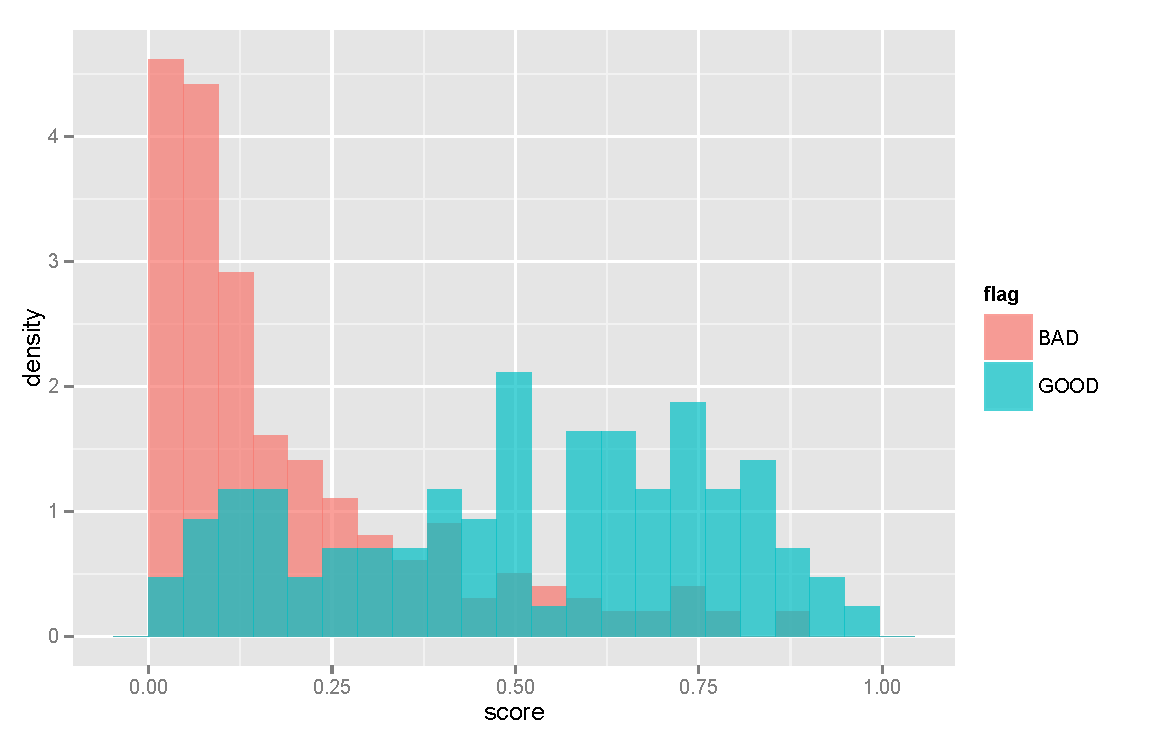
\includegraphics[width=\textwidth]{Plots/HIST_GLM}
                \label{fig:HIST_ GLM}
        \end{subfigure}

        \caption{Plot of Roc curve and histogram for GLM method}\label{fig:GLM}
\end{figure}

Another two plots - ROC curve and histogram can give us better understanding of the model performance. AUROC with value 0.83 is said to be really good. Interesting is that most of the bad values having very small score values. 

All simulations in this section had been done for the testing data sets.

\clearpage


\subsection{Scorecard for Logistic Regression}

\begin{table}[ht]
\centering
\begin{tabular}{rlr}
\hline
& Variable & Value \\ 
\hline
1 & (Intercept) & 511.93 \\ 
2 & `CHK\_ACCT$>$=200 DM` & -30.32 \\ 
3 & `CHK\_ACCT0-200 DM` & -14.95 \\ 
4 & `CHK\_ACCTno checking account` & -50.64 \\ 
5 & `DURATION\_TO\_AGE01 DURATION\_TO\_AGE $<$= 1.21875` & 26.56 \\ 
6 & `DURATION\_TO\_AGE02 DURATION\_TO\_AGE $<$= 3` & 67.92 \\ 
7 & `HISTORYcritical account/ other credits existing (not at this bank)` & -52.15 \\ 
8 & `HISTORYdelay in paying off in the past` & -37.21 \\ 
9 & `HISTORYexisting credits paid back duly till now` & -36.26 \\ 
10 & `HISTORYno credits taken/ all credits paid back duly` & -6.03 \\ 
11 & `DURATION01 DURATION $<$= 33` & 12.13 \\ 
12 & `DURATION02 DURATION $<$= 72` & 2.37 \\ 
13 & `AMOUNT01 AMOUNT $<$= 3913` & -59.83 \\ 
14 & `AMOUNT02 AMOUNT $<$= 7824` & 14.85 \\ 
15 & `AMOUNT03 AMOUNT $<$= 18424` & 47.81 \\ 
16 & `SAVINGS\_ACCT$>$=1000 DM` & -28.61 \\ 
17 & `SAVINGS\_ACCT100-500 DM` & -1.22 \\ 
18 & `SAVINGS\_ACCT500-1000 DM` & -14.45 \\ 
19 & `SAVINGS\_ACCTunknown/ no savings account` & -30.90 \\ 
20 & `PURPOSEcar (new)` & 16.19 \\ 
21 & `PURPOSEcar (used)` & -20.29 \\ 
22 & PURPOSEeducation & 31.75 \\ 
23 & `PURPOSEfurniture/equip\_domestic applia` & 11.91 \\ 
24 & PURPOSEothers & -10.23 \\ 
25 & `PURPOSEradio/television` & -4.87 \\ 
26 & PURPOSErepairs & 12.99 \\ 
27 & PURPOSEretraining & -50.63 \\ 
28 & `AMOUNT\_TO\_DURATION01 AMOUNT\_TO\_DURATION $<$= 250.944444444444` & -24.12 \\ 
29 & `AMOUNT\_TO\_DURATION02 AMOUNT\_TO\_DURATION $<$= 291.583333333333` & -48.23 \\ 
30 & `AMOUNT\_TO\_DURATION03 AMOUNT\_TO\_DURATION $<$= 358.090909090909` & -54.94 \\ 
31 & `AMOUNT\_TO\_DURATION04 AMOUNT\_TO\_DURATION $<$= 2482.66666666667` & 3.82 \\ 
\hline
\end{tabular}
\caption{Scorecard table} 
\end{table} 
 
 
 Scorecard gives us some information about contribution of single variables in the model. The bigger value off the score the bigger chance of client to be good. The calibration for this scorecard is standard wich means that for point value of 500 chance for being good is 0.5.
 
 Big contribution in this scorecard has for example AMOUNT. However interesting is that middle Amount gets the most points and oth smaller and bigger are worse. 
 
Here is important to note that for models in this section excluding Random Forest and Boosting the same variablees set had been used as for Logistic Regression.  
 \clearpage

\subsection{Linear Dyscryminant Analysis}

\begin{figure}[h!]
  \centering
  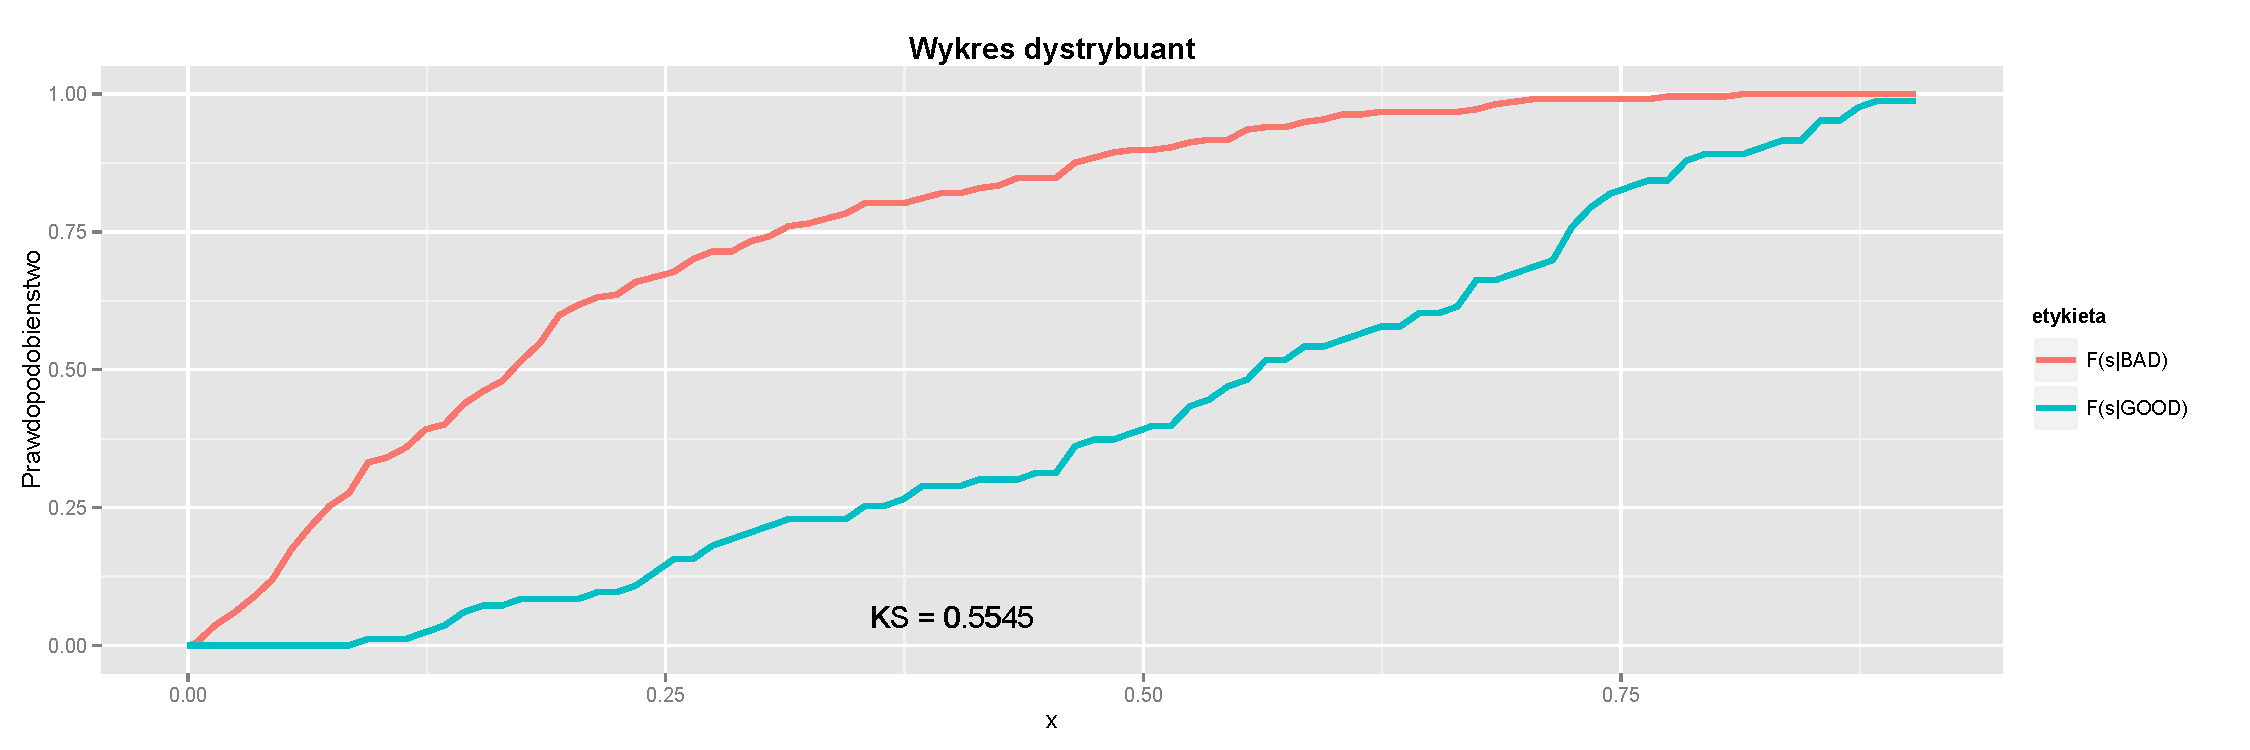
\includegraphics[width=0.9\textwidth]{Plots/LDA_KS}
  \caption[Close up of \textit{Hemidactylus} sp.]
   {Distribution plot for good and Bad class with KS statistic for LDA method}
\end{figure}

 It is also important to be addressed that the data for this model had been transformated into the WOE. It is also assumed that appropriate assumptions are fulfilled. With the value of KS styatistics 0.5545, LDA gives much better results than Logistic Regression. 

\begin{figure}[h!]
        \centering
        \begin{subfigure}[b]{0.45\textwidth}
                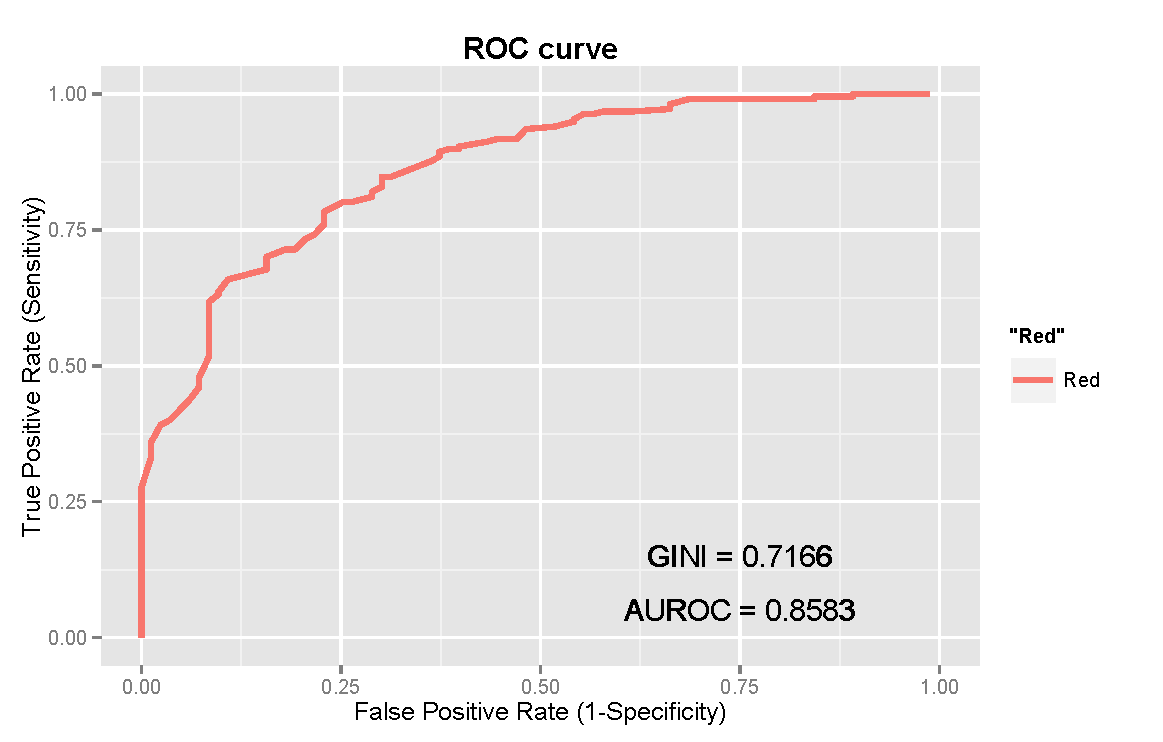
\includegraphics[width=\textwidth]{Plots/ROC_LDA}
                \caption{}
                \label{fig:ROC_ LDA}
        \end{subfigure}
        \begin{subfigure}[b]{0.45\textwidth}
                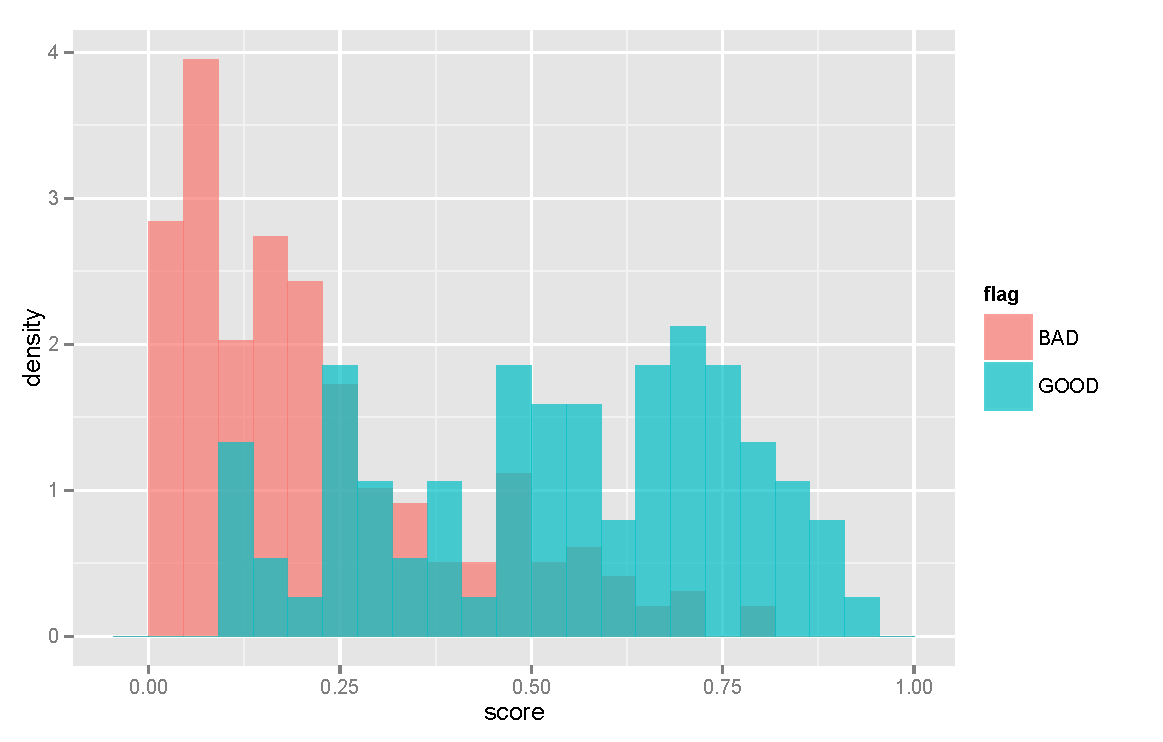
\includegraphics[width=\textwidth]{Plots/HIST_LDA}
                \label{fig:HIST_ LDA}
        \end{subfigure}

        \caption{Plot of Roc curve and histogram for LDA method}\label{fig:LDA}
\end{figure}


ROC curve also gives better results. AUROC statistic is equal 0.8583 which is very high. For the histogram interestting is that for two smallest classes there is no good observation in the bands. The same there is no bad observations for very large scores.



\clearpage

\subsection{KNN Method}

\begin{figure}[h!]
  \centering
  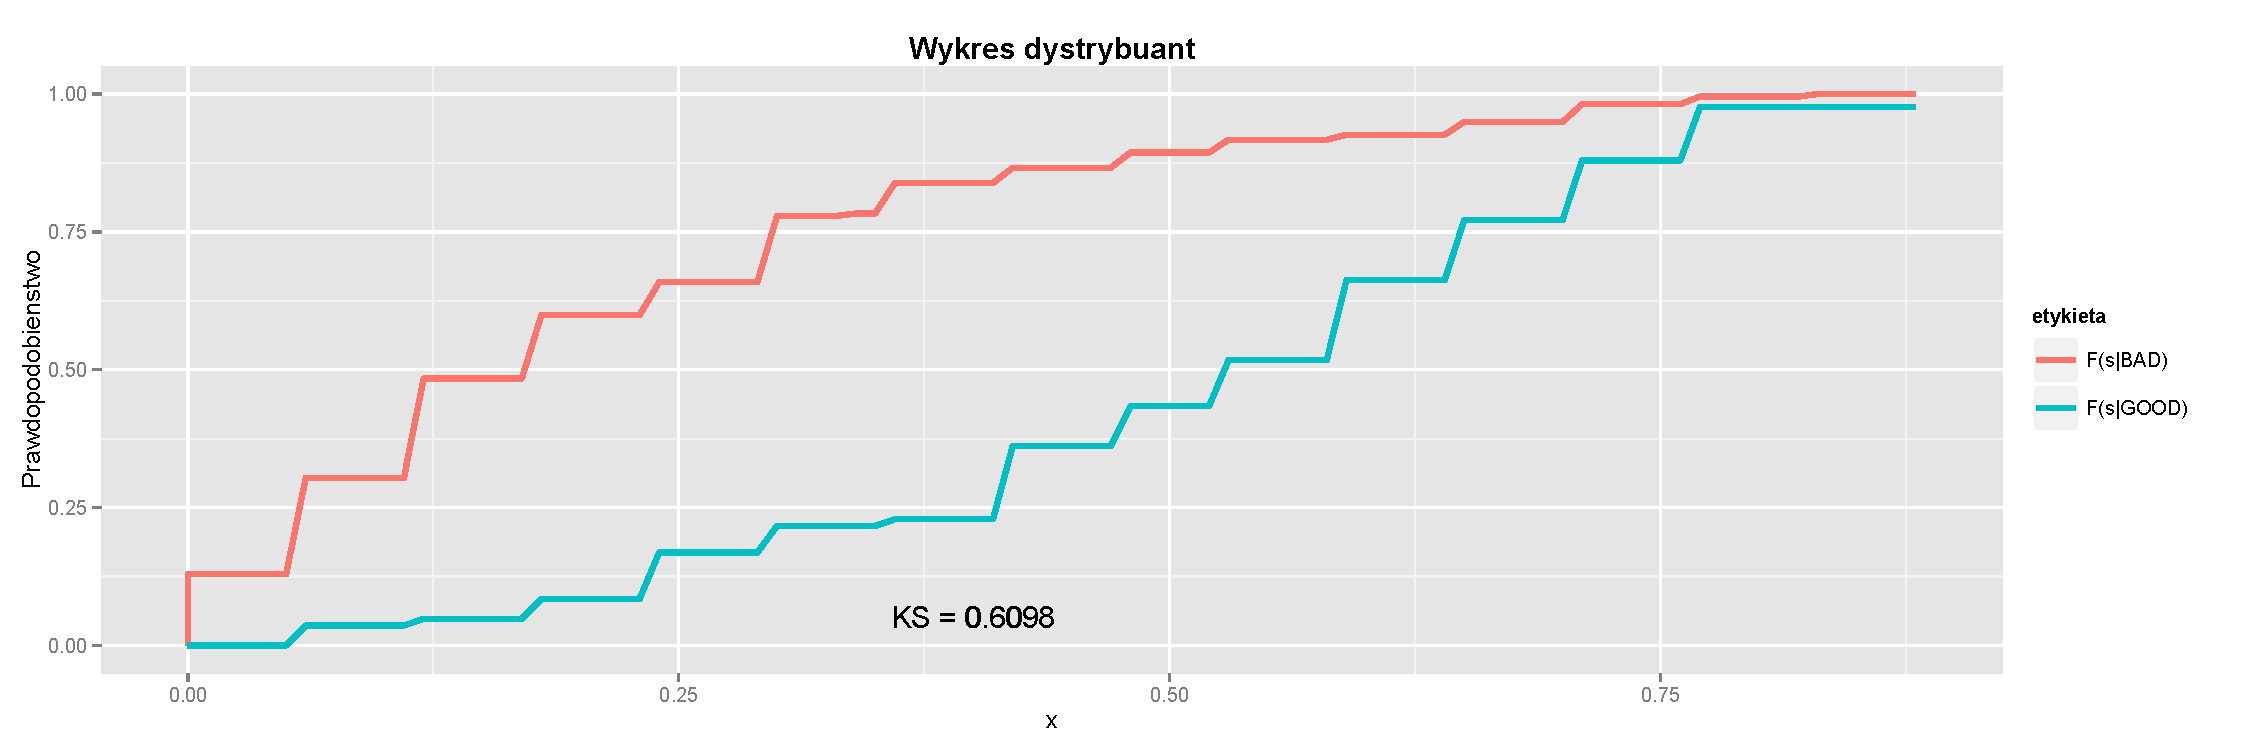
\includegraphics[width=0.9\textwidth]{Plots/KNN_KS}
  \caption[Close up of \textit{Hemidactylus} sp.]
   {Distribution plot for good and Bad class with KS statistic for KNN method}
\end{figure}

Similarily to the LDA method, KNN had been produced using WOE transformation of the data. The set of features is choosen to be the best for this task. nonethelss, estimation for the all predictor variables included gave better results. This could have effected in long time of computation for bigger data sets. 

\begin{figure}[h!]
        \centering
        \begin{subfigure}[b]{0.45\textwidth}
                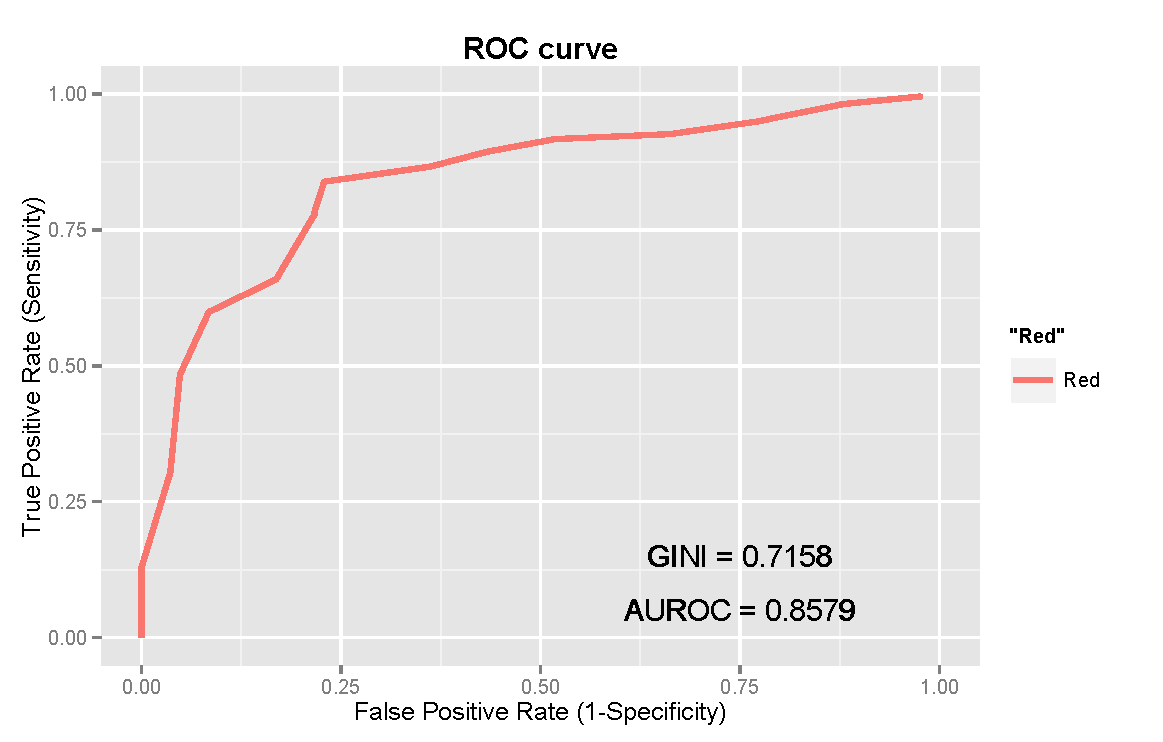
\includegraphics[width=\textwidth]{Plots/ROC_KNN}
                \caption{}
                \label{fig:ROC_ KNN}
        \end{subfigure}
        \begin{subfigure}[b]{0.45\textwidth}
                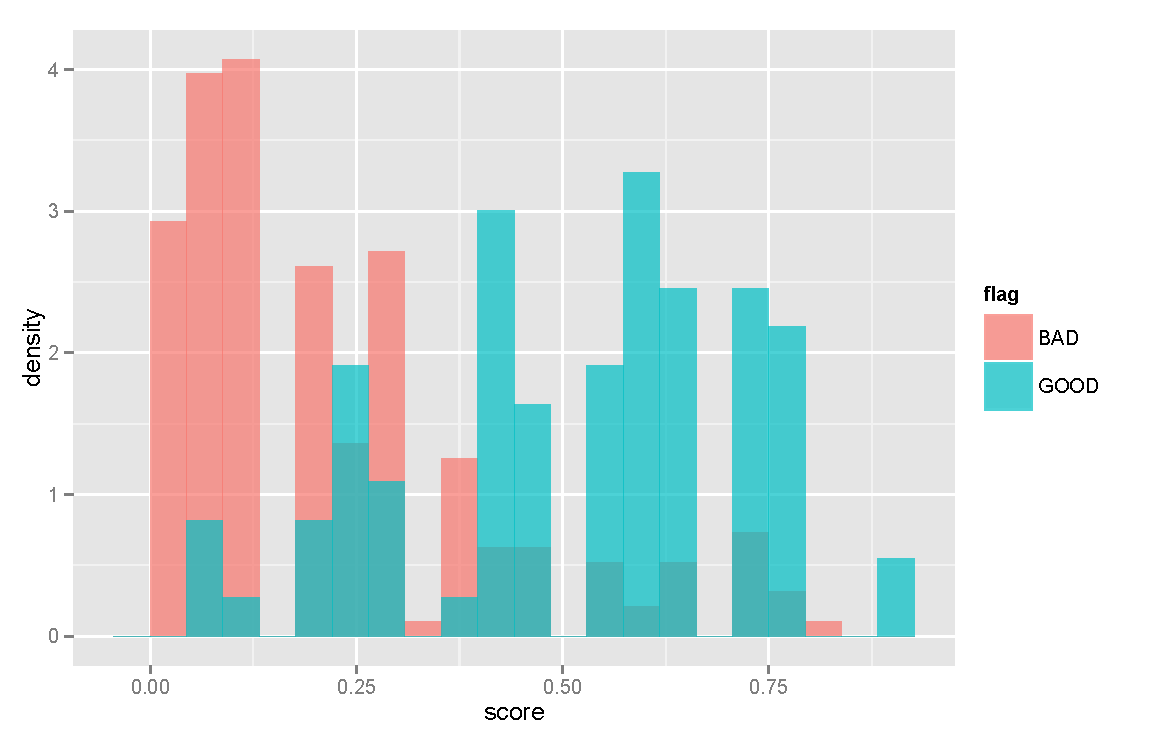
\includegraphics[width=\textwidth]{Plots/HIST_KNN}
                \label{fig:HIST_ KNN}
        \end{subfigure}

        \caption{Plot of Roc curve and histogram for KNN method}\label{fig:KNN}
\end{figure}

On the histogram we could observe sparse bins. It is caused by small number of different possible differences between distances for different observations. AUROC value is moderatelly good. 



It is important to say that tuning of the number of neighbours used in this model had been performed using 10 times repeated 10-k fold crossvalidation. The best model had been one with 19 neighbours. 

\clearpage

\begin{figure}[h!]
  \centering
  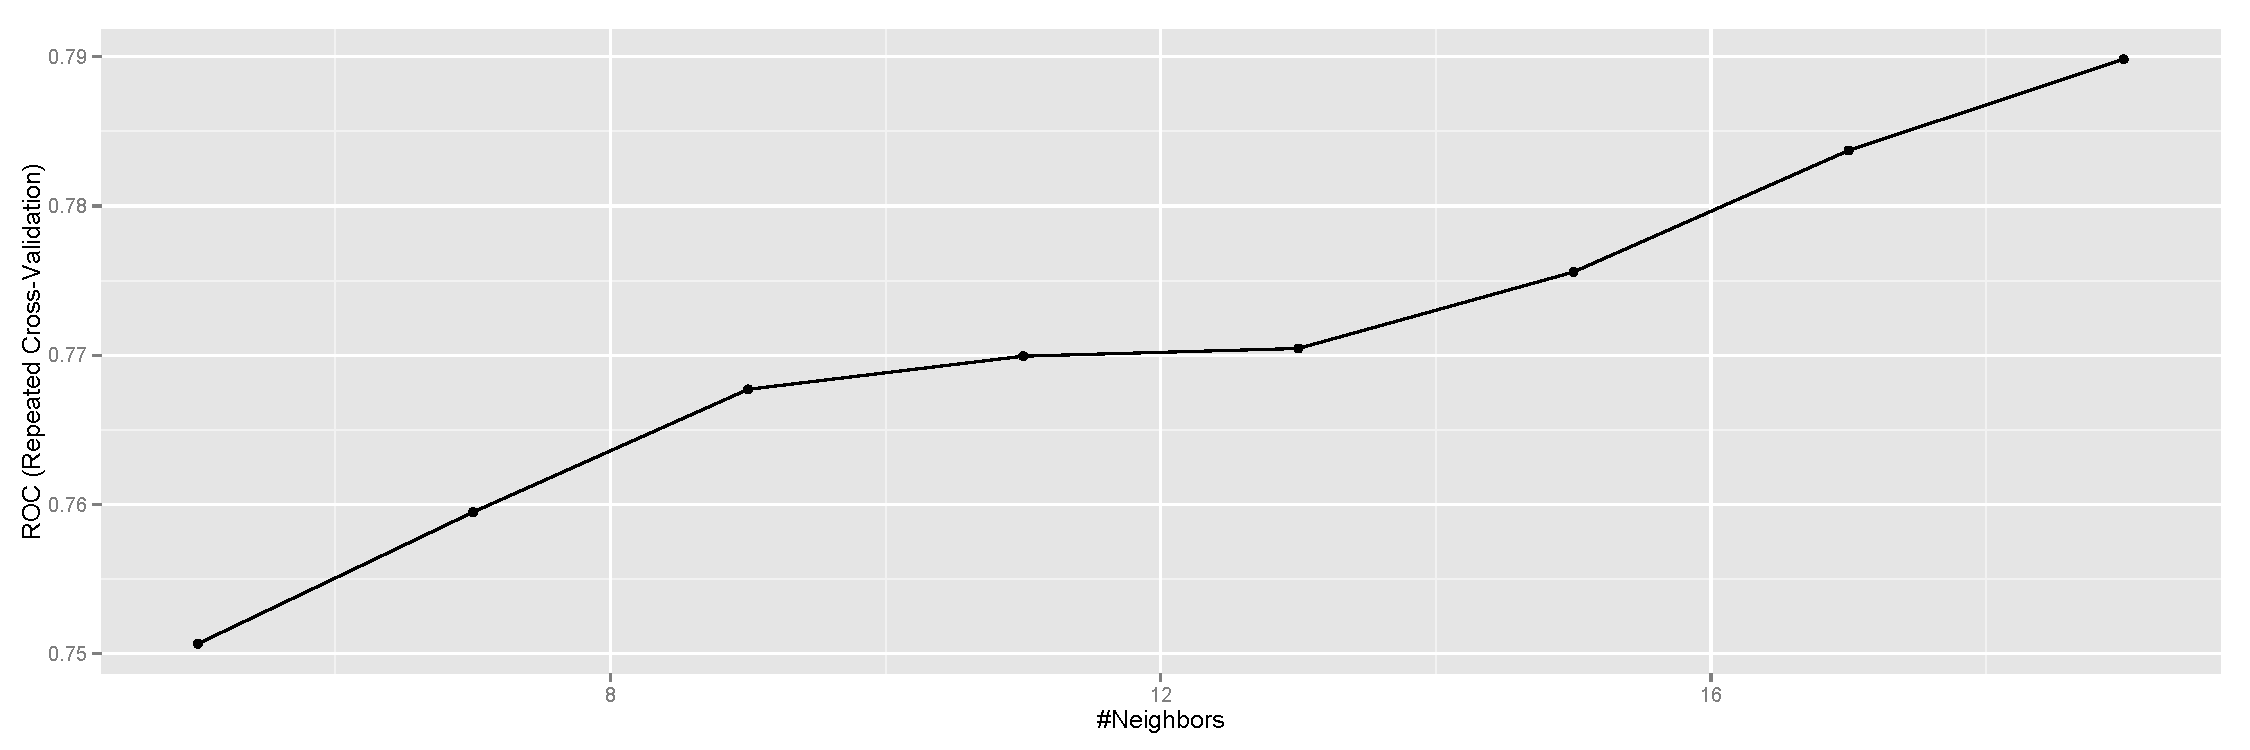
\includegraphics[width=0.9\textwidth]{Plots/TUNE_KNN}
  \caption
   {Tuning of the nieghbours number ROC results}
\end{figure}

Trend for different number of neighbours is visible upsising. We can expect that for bigger number, algorithm could have even better results, However for 700 observations in the training set, bigger number of observations could lead to overfitting of the model. Differences in the models performance are visible but not extrime. 

\subsection{Random Forest}

\begin{figure}[h!]
  \centering
  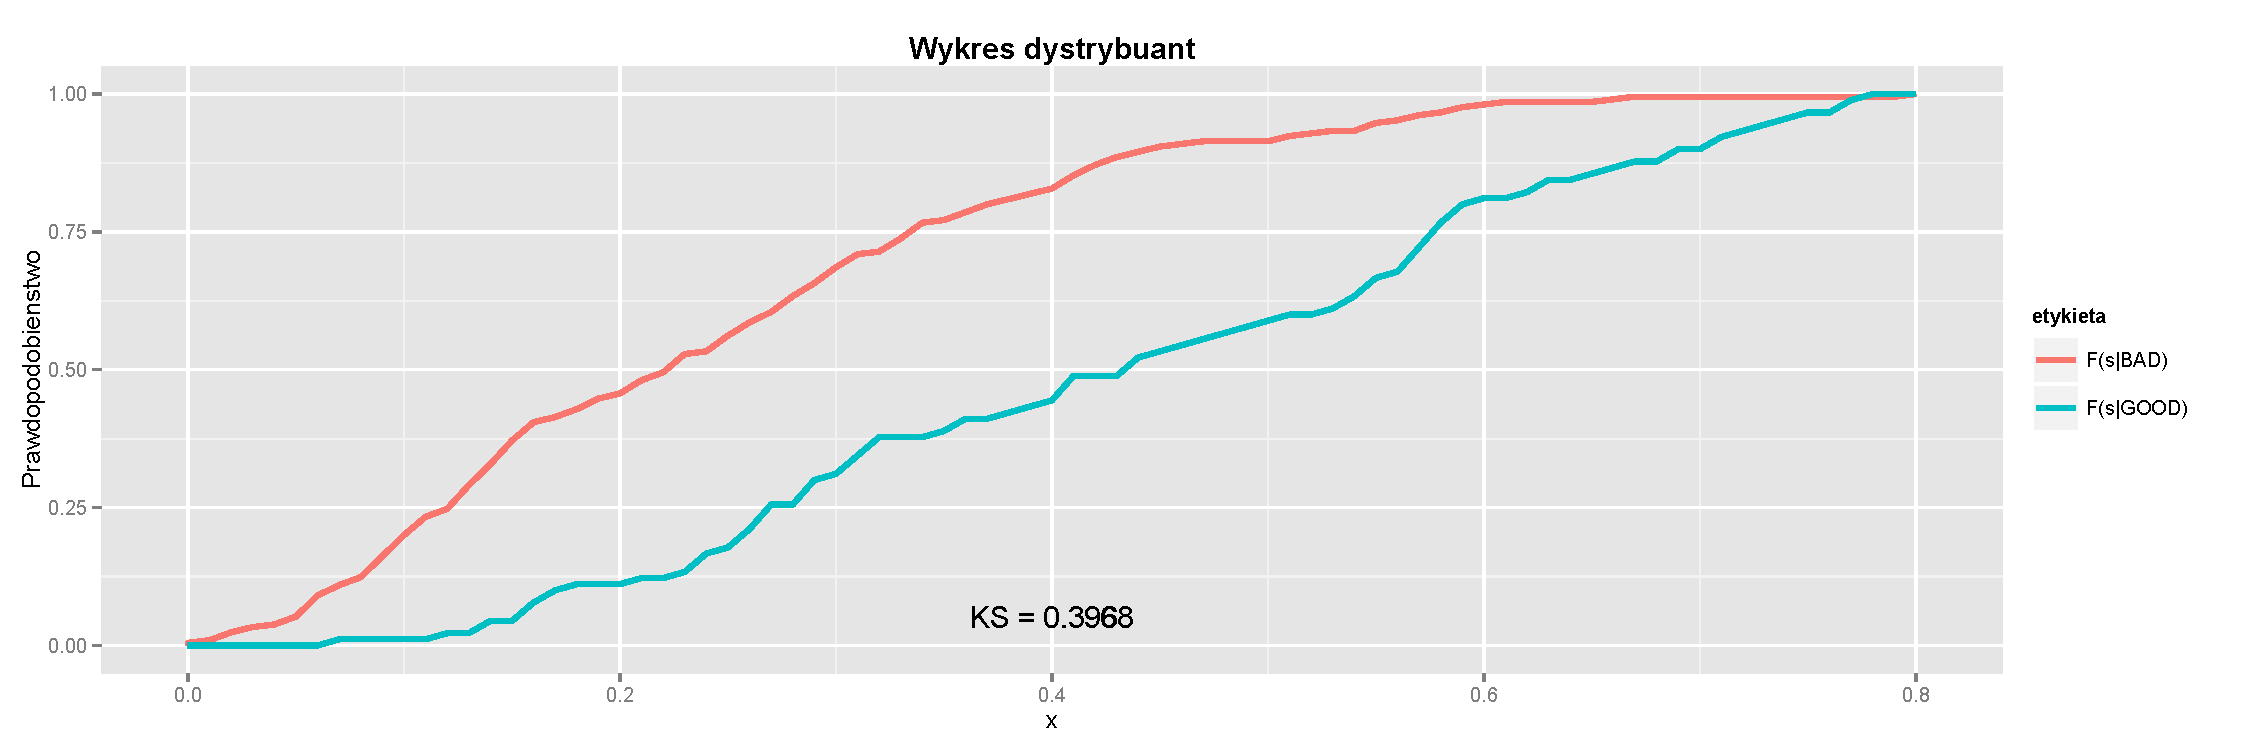
\includegraphics[width=0.9\textwidth]{Plots/RF_KS}
  \caption[Close up of \textit{Hemidactylus} sp.]
   {Distribution plot for good and Bad class with KS statistic for RF method}
\end{figure}

Suprising fact is that random forest model is behaving not to good. Separation based on the KS statistic is very weak and much worse than simple logistic regression. It could be caused also by over fitting for this model. 
Even though it is overfitted it performs moderately well. 

\clearpage

\begin{figure}[h!]
        \centering
        \begin{subfigure}[b]{0.45\textwidth}
                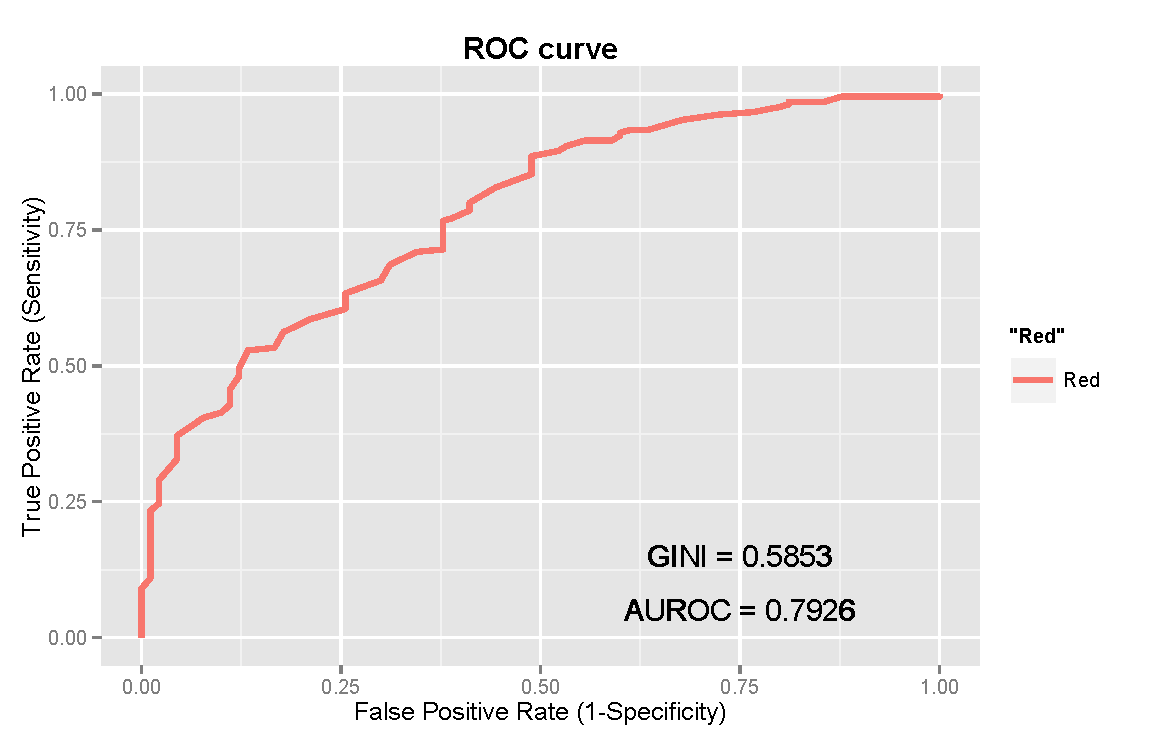
\includegraphics[width=\textwidth]{Plots/ROC_RF}
                \caption{}
                \label{fig:ROC_ RF}
        \end{subfigure}
        \begin{subfigure}[b]{0.45\textwidth}
                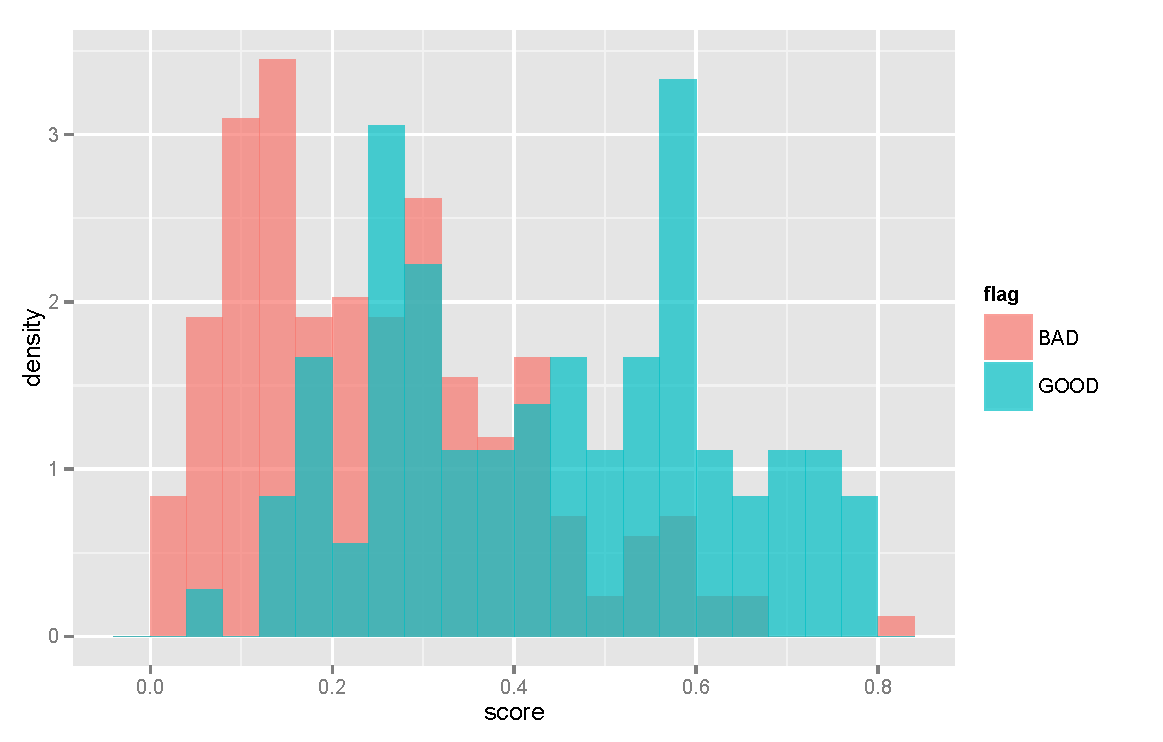
\includegraphics[width=\textwidth]{Plots/HIST_RF}
                \label{fig:HIST_ RF}
        \end{subfigure}

        \caption{Plot of Roc curve and histogram for RF method}\label{fig:RF}
\end{figure}

For this figure we see aggain that comparing to the other models, RF gives bad results. On the histogrm, even for small score bands there is a lot of the Good observations. 

\begin{figure}[h!]
  \centering
  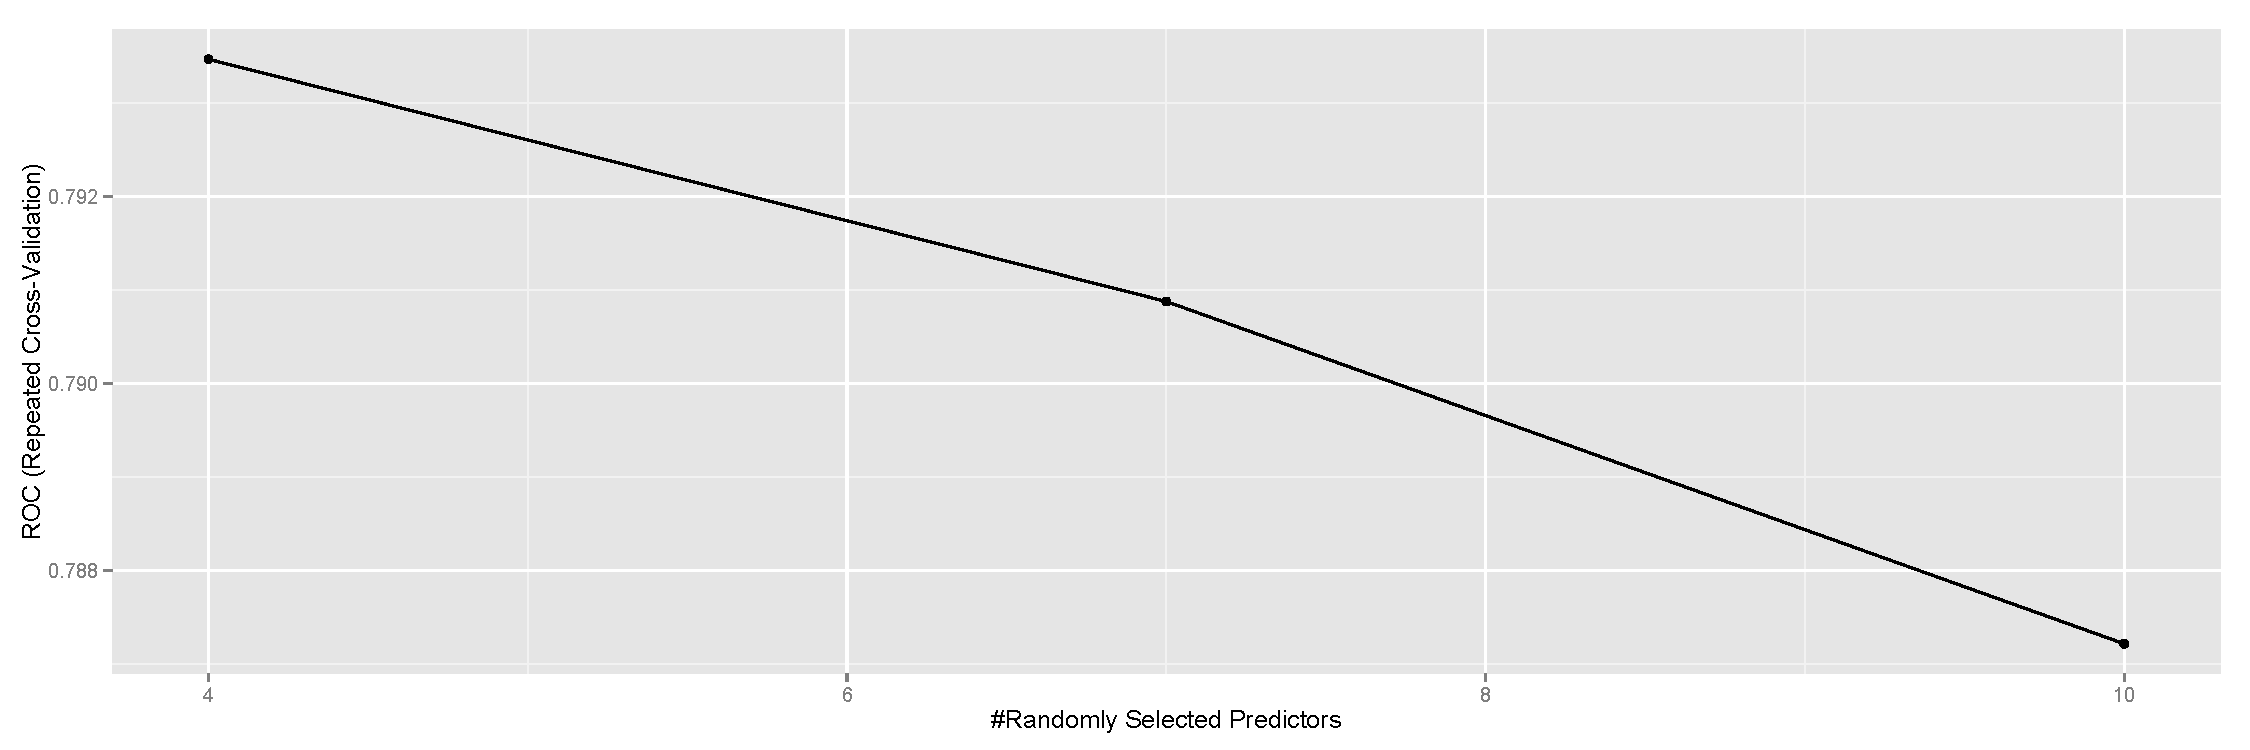
\includegraphics[width=0.9\textwidth]{Plots/TUNE_RF}
  \caption
   {Tuning of the trees number ROC results}
\end{figure}

Tuning is done similarily to the KNN model. There had been performed 10 times repeated 10 fold crossvalidation. This figure shows that for the bigger number of the trees for single step the power of the model is falling. It shows also that the best model and at the same time final model had been one with the 4 features sampeled at each time. 

\clearpage

\section{Boosting}

Boosting is another benchmark method. It had not been considered at beggining but as a extremaly good considered method it would serve as benchmark to compare with the other methods improved with the feature selection. For this method ther was no step of feature selection. Model had been tuned and calculated for the full data set. 

\begin{figure}[h!]
  \centering
  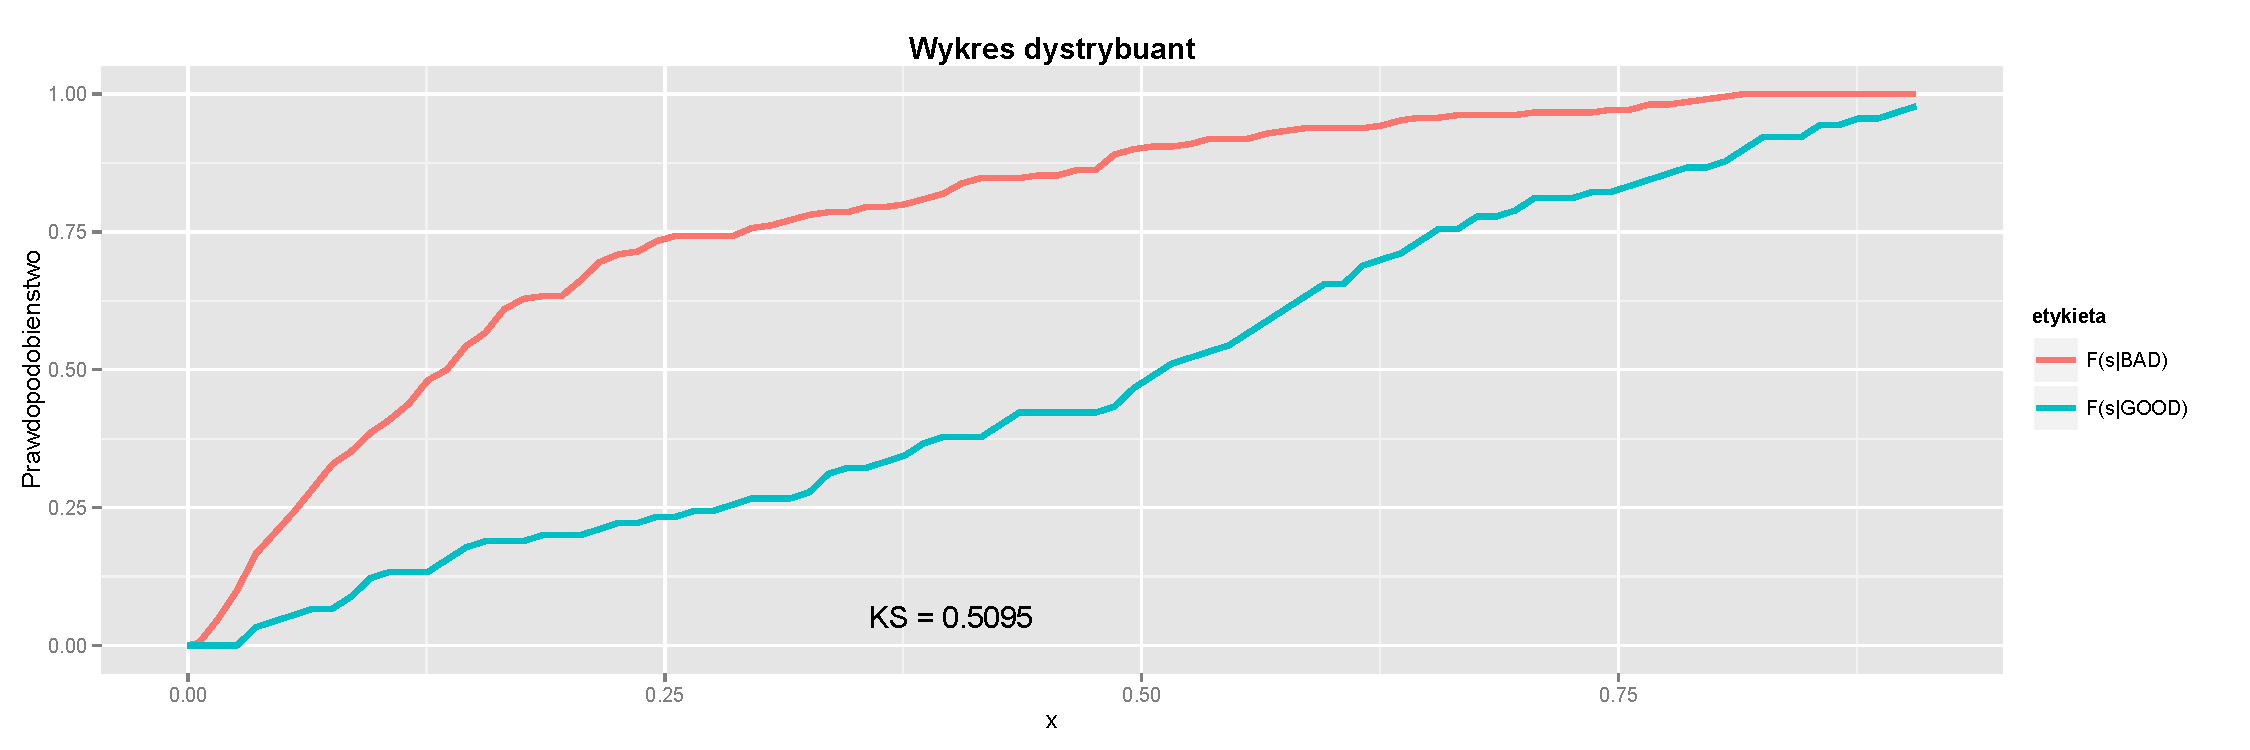
\includegraphics[width=0.9\textwidth]{Plots/GBM_KS}
  \caption[Close up of \textit{Hemidactylus} sp.]
   {Distribution plot for good and Bad class with KS statistic for GBM method}
\end{figure}


Similarily with the Random Forestt method in this case results are not too good comparing with other methods. Although the KS Value is better than for the RF, it is still smaller than any other method with performed feature selection. 

\begin{figure}[h!]
        \centering
        \begin{subfigure}[b]{0.45\textwidth}
                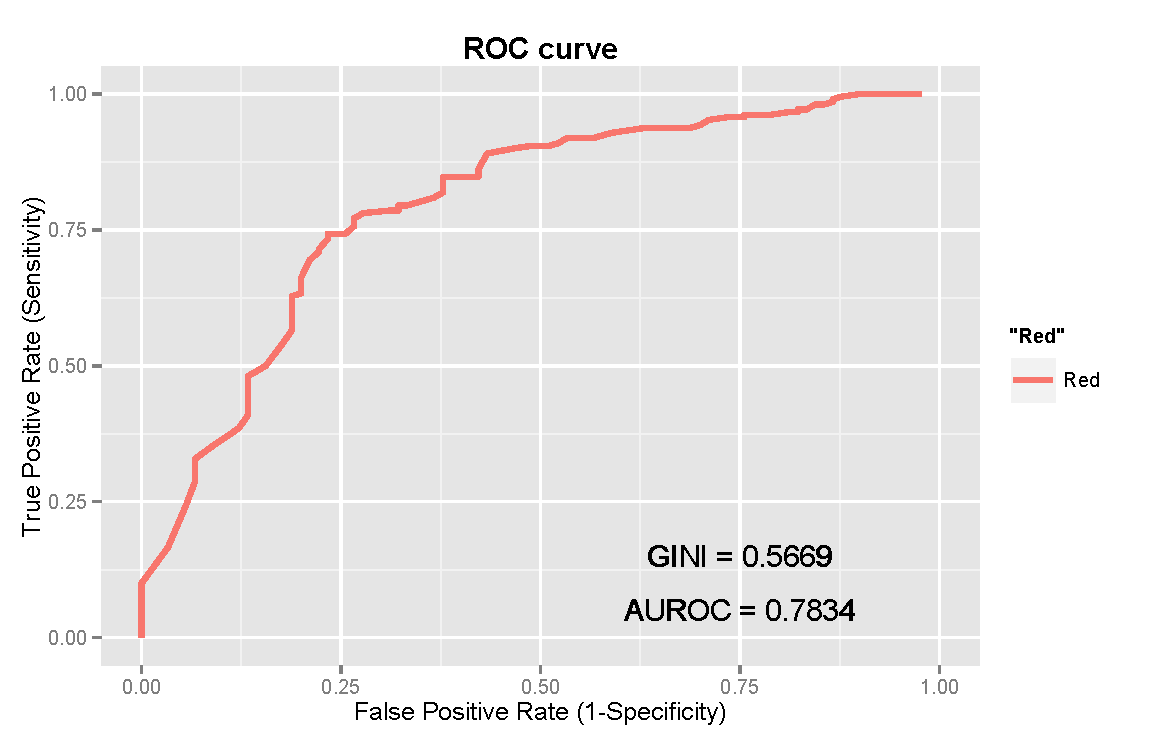
\includegraphics[width=\textwidth]{Plots/ROC_GBM}
                \caption{}
                \label{fig:ROC_ GBM}
        \end{subfigure}
        \begin{subfigure}[b]{0.45\textwidth}
                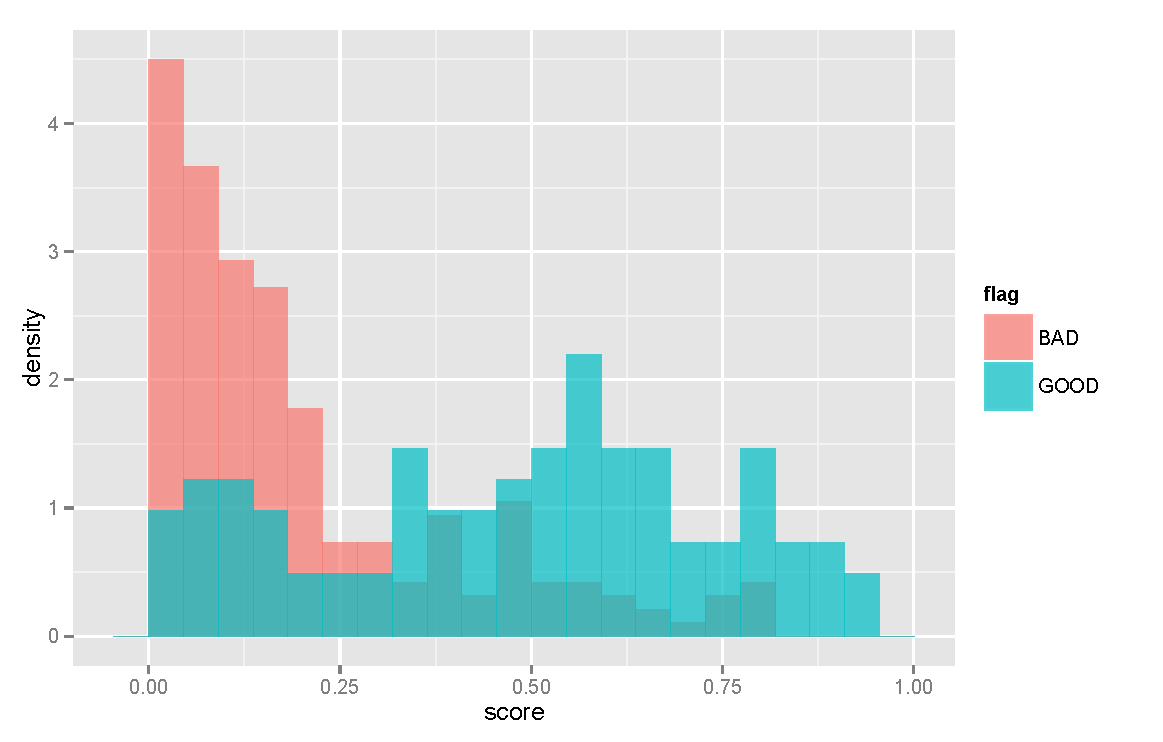
\includegraphics[width=\textwidth]{Plots/HIST_GBM}
                \label{fig:HIST_ GBM}
        \end{subfigure}

        \caption{Plot of Roc curve and histogram for GBM method}\label{fig:GBM}
\end{figure}


The histogram for this model is even worse than for the Random Forest. For first four scorebands number of Good observations is very high.  Value of AUROC is good.

\clearpage 

\begin{figure}[h!]
  \centering
  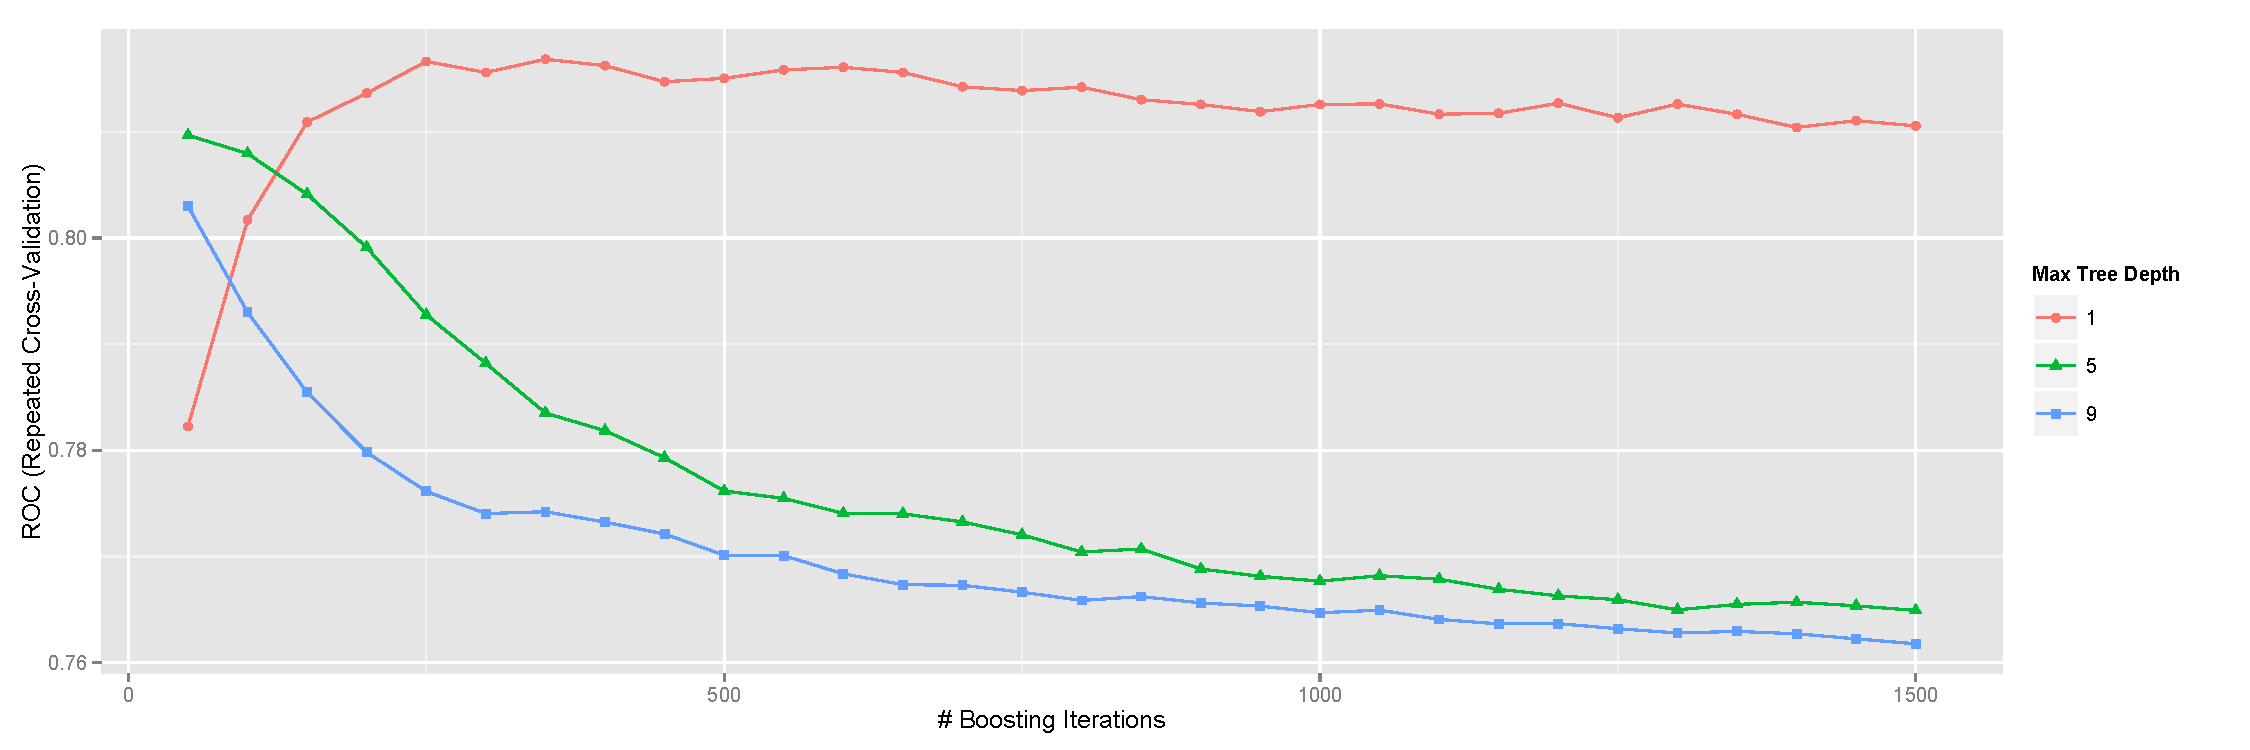
\includegraphics[width=0.9\textwidth]{Plots/TUNE_GBM}
  \caption
   {Tuning of the tree depth ROC results}
\end{figure}

For the boosting method there are two tuning parameters. Number of iterations in the algorithm and depth of the tree. We could see that for the deepth equal just one the results are the best. What is more, there is no significant improvement for bigger  iteration number than 500 for any algorithm. 

\begin{figure}[h!]
  \centering
  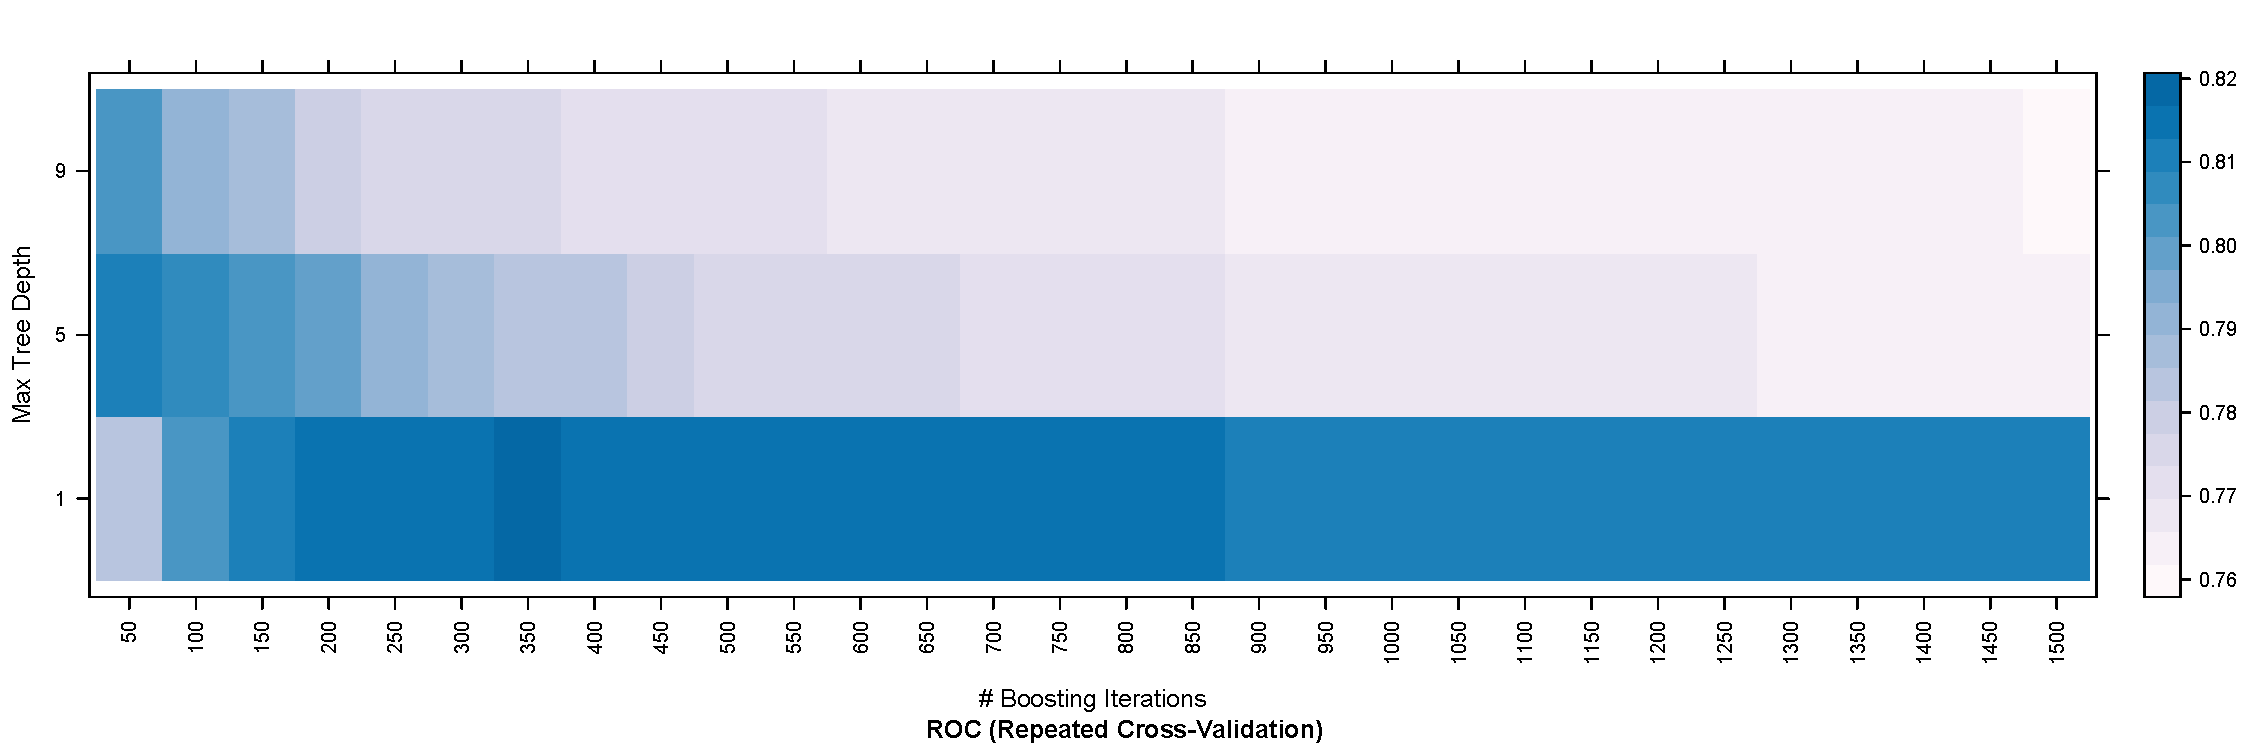
\includegraphics[width=0.9\textwidth]{Plots/TUNE_GBM_1}
  \caption
   {Tuning of the tree depth ROC results}
\end{figure}
  
What is more all of the algorithms are getting worse at some point. It could mean that for such values we start to overfit (the extrime observatioins are tried to be fitted better what results in drop of power of the algorithm.)
Best tune had been achieved for the 250 iterations with depth just 1. ROC for this setup is being estimated as around 0.8. oFor Bigger depths of the trees we expect big overfit. 

\clearpage

\subsection{Summary of Modeling and Feature Selection}

In last two sections there had been many interesting patterns discovered. The most interestting results sre that:

\begin{itemize}

\item Ofen including not relevant predictors in the data set could effect in the loss of the power for the model.

\item Even for very small predictors set, results could be very optimistic as it had been shown for CFS set of features. 

\item Proper feature selection can boost Logistic Regressioin to be better than methods with automatic feature selection and parameter tuning. 

\item Using Scorecard interesting relations within the data can be discovered. It also sometime can be used to manipulate with the score. For example what happened if I am Married , would I get higher or lower credit offer. 

\end{itemize}


\clearpage

\clearpage
 
\section{Cluster analysis results}


\clearpage
\section{Summary}



% ==============================================================================
% ==============================================================================
% ==============================================================================
\clearpage
\part{Discussion}






% ==============================================================================
% ==============================================================================
% ==============================================================================
\clearpage
\begin{thebibliography}{99}
\bibitem{} Computational Methods of Feature Selection (Chapman \& Hall/CRC Data Mining and Knowledge Discovery Series), Huan Liu, Hiroshi Motoda, 2007, ISBN-13: 978-1584888789  
\bibitem{} Hall, M. A., Smith, L. A. (1998). Practical feature subset selection for machine learning. Australian Computer Science Conference. Springer. 181-191.
\bibitem{} Liu, H. and Setiono, R., Chi2: Feature selection and discretization of numeric attributes, Proc. IEEE 7th International Conference on Tools with Artificial Intelligence, 338-391, 1995
\bibitem{} R.C. Holte (1993). Very simple classification rules perform well on most commonly used datasets. Machine Learning. 11:63-91.
\bibitem{} Kenji Kira, Larry A. Rendell: A Practical Approach to Feature Selection. In: Ninth International Workshop on Machine Learning, 249-256, 1992.
\bibitem{} Igor Kononenko: Estimating Attributes: Analysis and Extensions of RELIEF. In: European Conference on Machine Learning, 171-182, 1994.
\bibitem{} Marko Robnik-Sikonja, Igor Kononenko: An adaptation of Relief for attribute estimation in regression. In: Fourteenth International Conference on Machine Learning, 296-304, 1997.
\bibitem{} StatSoft, Formula Guide Weight of Evidence Module http://documentation.statsoft.com/portals/0/formula%20guide/Weight%20of%20Evidence%20Formula%20Guide.pdf
\bibitem{} Data Clustering: A Review, A.K. Jain, M.N. Murty, P.J. Flynn, 1999, https://www.cs.rutgers.edu/~mlittman/courses/lightai03/jain99data.pdf
\bibitem{} Principal component analysis From Wikipedia, the free encyclopedia, http://en.wikipedia.org/wiki/Principal\_component\_analysis
\bibitem{} notes from Laboratory for Dynamic Synthetic Vegephenonenology (LabDSV),
the University of California, http://ecology.msu.montana.edu/labdsv/R/labs/
\bibitem{} clValid, an R package for cluster validation, Guy Brock, Vasyl Pihur, Susmita Datta, and Somnath Datta, Department of Bioinformatics and Biostatistics, University of Louisville, http://cran.r-project.org/web/packages/clValid/vignettes/clValid.pdf
\end{thebibliography}

\end{document}
